%%
%% Copyright 2007, 2008, 2009 Elsevier Ltd
%%
%% This file is part of the 'Elsarticle Bundle'.
%% ---------------------------------------------
%%
%% It may be distributed under the conditions of the LaTeX Project Public
%% License, either version 1.2 of this license or (at your option) any
%% later version.  The latest version of this license is in
%%    http://www.latex-project.org/lppl.txt
%% and version 1.2 or later is part of all distributions of LaTeX
%% version 1999/12/01 or later.
%%
%% The list of all files belonging to the 'Elsarticle Bundle' is
%% given in the file `manifest.txt'.
%%

%% Template article for Elsevier's document class `elsarticle'
%% with numbered style bibliographic references
%% SP 2008/03/01
%%
%%
%%
%% $Id: elsarticle-template-num.tex 4 2009-10-24 08:22:58Z rishi $
%%
%%
\documentclass[preprint,12pt]{elsarticle}

%% Use the option review to obtain double line spacing
%% \documentclass[preprint,review,12pt]{elsarticle}

%% Use the options 1p,twocolumn; 3p; 3p,twocolumn; 5p; or 5p,twocolumn
%% for a journal layout:
%% \documentclass[final,1p,times]{elsarticle}
%% \documentclass[final,1p,times,twocolumn]{elsarticle}
%% \documentclass[final,3p,times]{elsarticle}
%% \documentclass[final,3p,times,twocolumn]{elsarticle}
%% \documentclass[final,5p,times]{elsarticle}
%% \documentclass[final,5p,times,twocolumn]{elsarticle}

%% if you use PostScript figures in your article
%% use the graphics package for simple commands
%% \usepackage{graphics}
%% or use the graphicx package for more complicated commands
%% \usepackage{graphicx}
%% or use the epsfig package if you prefer to use the old commands
%% \usepackage{epsfig}

%% The amssymb package provides various useful mathematical symbols
\usepackage{amssymb}
\usepackage{xcolor}

%\ifCLASSINFOpdf
%\usepackage[pdftex]{graphicx}
%% declare the path(s) where your graphic files are
%%\graphicspath{{../pdf/}{../jpeg/}}
%\graphicspath{{images/}}
%% and their extensions so you won't have to specify these with
%% every instance of \includegraphics
%% \DeclareGraphicsExtensions{.pdf,.jpeg,.png}
%\else
%% The amsthm package provides extended theorem environments
%% \usepackage{amsthm}
\usepackage{amsmath}
%\usepackage{calrsfs}
%\usepackage{bm}
\usepackage{amssymb}
\usepackage{array}
\usepackage{tabu}
\usepackage{float}
\usepackage{svg}
%\usepackage[]{algorithm2e}
%\usepackage{algorithm}
%\usepackage[]{algorithmic}
\usepackage{algorithm, algorithmic}
%\usepackage[colorlinks]{hyperref}
\usepackage{xcolor}

\newcolumntype{M}[1]{>{\centering\arraybackslash}m{#1}}
\newcolumntype{N}{@{}m{0pt}@{}}


\newcommand\norm[1]{\left\lVert#1\right\rVert}

\newcommand{\trans}{\mathsf{T}}


%% The lineno packages adds line numbers. Start line numbering with
%% \begin{linenumbers}, end it with \end{linenumbers}. Or switch it on
%% for the whole article with \linenumbers after \end{frontmatter}.
%% \usepackage{lineno}

%% natbib.sty is loaded by default. However, natbib options can be
%% provided with \biboptions{...} command. Following options are
%% valid:

%%   round  -  round parentheses are used (default)
%%   square -  square brackets are used   [option]
%%   curly  -  curly braces are used      {option}
%%   angle  -  angle brackets are used    <option>
%%   semicolon  -  multiple citations separated by semi-colon
%%   colon  - same as semicolon, an earlier confusion
%%   comma  -  separated by comma
%%   numbers-  selects numerical citations
%%   super  -  numerical citations as superscripts
%%   sort   -  sorts multiple citations according to order in ref. list
%%   sort&compress   -  like sort, but also compresses numerical citations
%%   compress - compresses without sorting
%%
%% \biboptions{comma,round}

% \biboptions{}


\journal{}
\graphicspath{{images/}}

\begin{document}
	
	\begin{frontmatter}
		
		%% Title, authors and addresses
		
		%% use the tnoteref command within \title for footnotes;
		%% use the tnotetext command for the associated footnote;
		%% use the fnref command within \author or \address for footnotes;
		%% use the fntext command for the associated footnote;
		%% use the corref command within \author for corresponding author footnotes;
		%% use the cortext command for the associated footnote;
		%% use the ead command for the email address,
		%% and the form \ead[url] for the home page:
		%%
		%\title{k km kmkmkm\tnoteref{label1}}
		%\tnotetext[label1]{}
		\author{Ali Noroozi}
		\author{Mansoor rezghi\corref{cor1}\fnref{label2}}
		\ead{Rezghi@modares.ac.ir}
		%\ead[url]{home page}
		% \fntext[label2]{}
		% \cortext[cor1]{}
		\address{Department of Computer Science, Tarbiat Modares University, Tehran-Iran\fnref{label3}}
		%\fntext[label3]{}
		
		\title{A Tensor Framework for Alzheimer's Disease early Detection and Functional Connectivity Analysis in Resting State fMRI}
		
		%% use optional labels to link authors explicitly to addresses:
		%% \author[label1,label2]{<author name>}
		%% \address[label1]{<address>}
		%% \address[label2]{<address>}
		
		
		
		\address{}
		
		\begin{abstract}
			%% Text of abstract
			
			Recently machine learning methods had gain lots of publicity among researchers
			in order to analyze the brain images such as Resting-State Functional
			Magnetic Resonance Imaging(rs-fMRI) to obtain a better understanding
			of the brain and its related disease such as Alzheimer’s disease. Finding
			the common patterns caused by a brain disorder through analyzing the
			functional connectivity(FC) network along with discriminating brain diseases
			from normal controls have traditionally been two main goals in studying rs-fMRI
			data. The majority of techniques for finding an FC, calculate the FC
			matrix for each subject and then use simple techniques in order to combine
			them to obtain general functional connectivity. Also, the states of the art classification
			techniques for finding subjects with brain disorders, also rely on
			calculating an FC for each subject, vectorize them and then feed them to
			the classifier. Considering these problems and based on multidimensional
			nature data, we have come up with a novel tensor framework in which the
			FC calculation for each class is done without the need to construct the FC
			for each sample, also this framework allows us to reduce the dimensionality,
			and create a novel discriminant function that avoids vectorization in any step
			and uses the test data in the training process without forcing any prior
			knowledge about its label to the classifier  
			Extensive experiments using the ADNI dataset demonstrate that
			our proposed framework effectively boosts the fMRI classification performance and reveals novel connectivity patterns in Alzheimer's disease at its early stages.
			%
			%Different methods have been deployed in order to discriminate Alzheimer's disease from normal ones which is a hard task, especially in early stages (eMCI) case. The majority of deployed techniques rely on constructing the functional connectivity (FC) for each person and use the vectorized FC as the input for the classifiers which has two main drawbacks: 1) The need for constructing the FC********The loss of possible valuable structural information in the vectorization step.
			%Considering these problems and based on multidimensional nature the data, we have came up with a novel framework which omits the FC construction part and preserve the structural integrity of data for the classification.
			%    The proposed framework uses the High Order Singular Value Decomposition (HOSVD) in order to prune the classes and select the proper basis for each of them.
			%This framework also allows us to obtain a general FC pattern for normal and eMCI classes but not a single sample which helps us to shed more lights on the brain abnormalities in the Alzheimers disease at its early stages. 
			%        Extensive experiments using the ADNI dataset demonstrate that
			%        our proposed framework effectively boosts the fMRI classification performance and reveals novel connectivity patterns in Alzheimer's disease at its early stages.
		\end{abstract}
		
		\begin{keyword}
			%% keywords here, in the form: keyword \sep keyword
			Tensor Decomposition, fMRI, Functional Connectivity
			%% MSC codes here, in the form: \MSC code \sep code
			%% or \MSC[2008] code \sep code (2000 is the default)
			
		\end{keyword}
		
	\end{frontmatter}
	
	%%
	%% Start line numbering here if you want
	%%
	% \linenumbers
	
	%% main text
	\section{Introduction}
	\label{Intro}
	Alzheimer’s disease (AD) is a progressive neurodegenerative disorder with a long pre-morbid asymptomatic period which affects millions of elderly individuals worldwide\cite{r01}. It is predicted that the number of affected people will double in the next 20 years, and 1 in 85 people will be affected by 2050 \cite{r02}. The predominant clinical symptoms of AD include a decline in some important brain cognitive and intellectual abilities, such as memory, thinking, and reasoning. Precise diagnosis of AD, especially at its early warning stage: early Mild Cognitive Impairment (eMCI), enables treatments to delay or even avoid such disorders \cite{r03}.
	
	In recent years, brain imaging techniques like Positron Emission Tomography (PET)\cite{r21}, Electroencephalography (EEG)\cite{r22}
	and functional Magnetic Resonance Imaging (fMRI)\cite{r23} 
	have been used in the analysis of AD. Due to the high spatial resolution and relatively lower costs, fMRI is vastly used among researchers in order to monitor brain activities especially in AD and all its stages in which detecting abnormalities within small brain regions is essential \cite{r04}. 
	An fMRI sample is naturally a 4D tensor consisting of 3D voxels moving in time, and each voxel contains an intensity value that is proportional to the strength of the Blood Oxygenation Level Dependent(BOLD) signal, which is a measure of the changes in blood flow, to estimate the activity of different brain regions\cite{r07}.
	Resting-state fMRI(rs-fMRI) is an fMRI technique in which the patient is asked to rest during the whole scan, focuses on the low-frequency $\left( < 0.1 Hz \right)$  oscillations of BOLD signal, which presents the underlying neuronal activation patterns of brain regions. rs-fMRI is usually used in order to analyze brain diseases like AD or Autism\cite{r33,r34}.
	%
	%Since the number of voxels within a single full scan is high 
	%($5000$ up to roughly $200,000$[ref(Definingnodes)]) and they form strong spatial relations, 
	
	Since each fMRI volume consist of hundreds of thousands of voxels which are often highly correlated with the surrounding voxels in the brain volume, parcellation of the brain for further analysis has moved toward the use
	of anatomical atlases. These atlases are strictly defined using
	anatomical features of the brain, like locations of common gyri
	and do not rely on any functional information.
	To generate data
	using an Atlas-based approach, the BOLD signal from all voxels is averaged within each brain region called Region of Interest(ROI)\cite{r09}.
	By putting together the average time-series for all the ROIs, the $i$th volume would become $X_i \in \mathbb{R}^{T \times R} , i = \{1,2,\cdots, S\}$ in which $R$, $T$ and $S$ are the number of ROIs, time points and samples respectively. 
	The process of obtaining such a matrix is shown in Figure \ref{g1.1}.% 
	\begin{figure*}[!t]
		\centering
		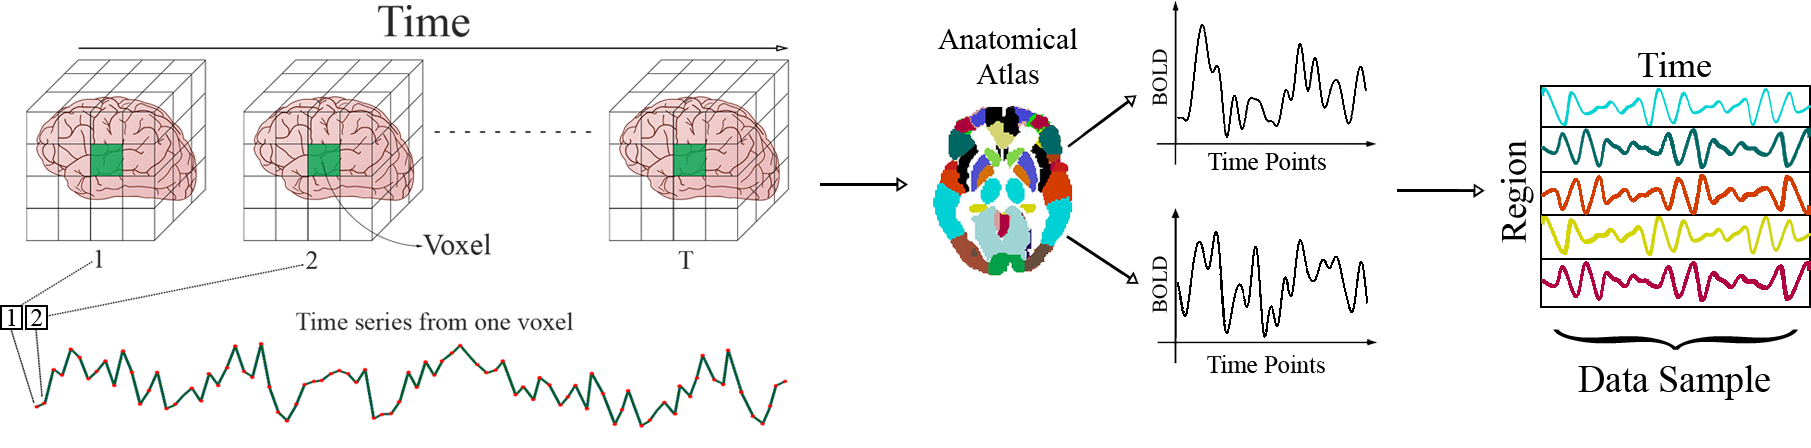
\includegraphics[width=5.5in]{Data}
		\caption{The process of extracting ROI time-series from the original 4D volume. }
		\label{g1.1}
	\end{figure*}
	
	%      There are two major studies associated with rs-fMRI data: finding common brain disorders caused by diseases like Alzheimer's or autism, and more recently detecting patients with brain disorders using classification techniques \cite{r35,r36}.
	%       Due to the high dimensionality of data and the nature of diseases like eMCI which does not show any reliable clinical symptoms,
	%        researchers moved towards advanced machine learning techniques in order to achieve more reliable analysis \cite{r37}.
	%        
	There are two major studies associated with rs-fMRI data: finding common brain disorders caused by diseases like Alzheimer's, Autism, schizophrenia and etc. and more recently detecting patients with brain disorders using classification techniques \cite{r35,r36}. Due to the high dimensionality of data and the nature of diseases like eMCI which does not show any reliable clinical symptoms,
	researchers moved towards advanced machine learning techniques in order to achieve more reliable analysis \cite{r37}.
	
	A powerful tool that is commonly used in order to achieve aforementioned goals is Functional Connectivity(FC) network.  FC is a $region \times region$ matrix $\bar{X}$ in which $\bar{x}_{ij}$ represents the functional connectivity between the $i$th and $j$th ROI. Functional connectivity is an observable
	phenomenon quantifiable with measures of statistical dependencies, such as correlations, coherence, or transfer entropy \cite{r38}.  Recent studies have shown that some brain disorders like AD could alter the way that some brain regions interact with each other. For example, compared with the healthy, AD patients have been found decreased functional connectivity between the hippocampus and other brain regions, and MCI patients have been observed increased functional connectivity between the frontal lobe and other brain regions\cite{r04}.
	So, Finding an FC that highlights the patterns caused by a disease, i.e. a \textbf{General} functional connectivity, has been a common goal in the rs-fMRI study for a long time. Several approaches exist to find common patterns among different brain scans. Data-driven methods such as PCA have been proposed for this task \cite{r55}. But ultimately most of them rely on calculating a network for each volume which may overlook the role of noises or outliers within the data\cite{r53,r54}. 
	
	In recent years FCs are also used as features in classification. 
	So, instead of using $X_i$ as the $i^{th}$ sample,  corresponding  FC i.e. $\bar{X}_i$ is used as a feature. Although FCs show promising results, they bring their own challenges.  The computational cost of FC is usually high and also its quality massively affects the performance of the learning process. Also, Since the conventional classifiers like \textbf{S}upport \textbf{V}ector \textbf{M}achine(SVM) and or k-NN works on data in vector format, these matrix features should be vectorized in order be fed to these classifiers.
	This vectorization leads to high-dimensional vectors which produce poor performance due to the phenomena known as the Curse of Dimensionality. Alongside the curse of dimensionality, vectorization also destroys potential information that is embedded in the structure of data. 
	This problem has been studied especially in image data in which vectorization destroys the spatial relations within an image\cite{r60}.
	
	
	In this paper, based on high order tensor decomposition, we have created a framework in which the aforementioned goals i.e. finding a general FC and detecting a disorder via classification could be achieved via a single \textbf{H}igh \textbf{O}rder \textbf{S}ingular \textbf{V}alue \textbf{D}ecomposition (HOSVD) of each class.
	Here based on latent variables obtained by HOSVD a general representative pattern of FC for eMCI and Normal controls are obtained. 
	The majority of connectivity patterns detected by this method have been observed and studied in several separated types of research which shows the reliability and power of the proposed method. Along with these connections, we have also detected novel connectivities especially regarding the Cerebellum which is usually discarded in the analysis of AD.     
	The proposed classifier also outperforms state of the art eMCI classification methods. 
	
	Viewing each class as a tensor allows us to work with \textit{time} and \textit{region} features separately but simultaneously. This multilinear view
	ables us to design a proper dimension reduction relative to the nature of each feature along with a discriminant function based on linear regression on latent space of samples that uses the test data to enhance the quality of the training set without forcing any a prior knowledge to the classifier, a task which is not possible through well known classifiers like SVM, logistic regression or k-NN. It is also notable that the proposed discriminant function directly works with the $X_i$s as features. Having the FC calculation step omitted in classification not only heavily affects the computational performance of the method, but it also saves us from the troubles of FCs which will be discussed in the next section.   
	
	To verify our approach, we conduct an extensive experimental study on rs-fMRI data from the
	benchmark dataset ADNI
	\footnote{http://adni.loni.usc.edu/}.
	As will be seen, the results demonstrate the effectiveness and advantages of our method. Specifically, the proposed framework, not only grants us superior classification accuracy to that from other methods, but it is also much faster and more stable against different data selection schemes. We have also confirmed our achieved general FC matrix using empirical data on the eMCI and Normal functional connectivity patterns.							 
	\section{eMCI classification and FC construction techniques}\label{related_works}
	
	%%%%%%%%%%%%%%%%%%%%%%%%%%%%%%%%%%%%%%%%%%%%%%%
	%%%%%%%%%%%%%%%%%%%%%%%%%%%%%%%%%%%%%%%%%%%%%%%
	%	
	%	As it was discussed before, classification techniques have become a favorable method for Alzheimer disease early detection. early classification methods used $X_{i}$s as the representative for each subject and used them directly in the classification process\textcolor{red}{ref?}. 
	%	As the functional connectivity matrix gain popularity among researchers, the majority of these classification methods shifted towards classifying the functional connectivity matrices\textcolor{red}{add some references!!}. 
	%%%%%%%%%%%%%%%%%%%%%%%%%%%%%%%%%%%%%%%%%%%%%%%%%%%%%%
	%%%%%%%%%%%%%%%%%%%%%%%%%%%%%%%%%%%%%%%%%%%%%%%%%%%%%%
	As it was mentioned before, obtaining and classifying FC matrices have become the dominant approach towards eMCI analysis. 
	Variety of methods such as Pairwise Pearson’s correlation coefficient \cite{r10, r11}, sparse representation \cite{r10, r12, r13}  and \textbf{S}parse \textbf{I}nverse \textbf{C}ovariance \textbf{E}stimation (SICE)\cite{r15} exists to obtain an FC.
	While the first two are easy to understand and can capture pairwise functional relationship based on a pair of ROIs, the latter can account for more complex interactions among multiple ROIs, but the estimation of partial correlation involves an inversion of a covariance matrix, which may be ill-posed due to the singularity of the covariance matrix. 
	These methods result in vastly different networks\cite{r35}. On the other hand, computing the correlations, based on the entire time series of fMRI data simply measures the FC between ROIs with a scalar value, which is fixed across time. This actually implicitly hypothesizes the \textbf{Stationary} interaction patterns among ROIs which will result in a \textit{static functional connectivity} (sFC). As a result, this method may overlook the complex and dynamic interaction patterns among ROIs, which are essentially time-varying. In order to overcome this issue, \textbf{Non-stationary} methods have been proposed which results in more complex networks also known as dynamic functional connectivity (dFC)\cite{r16,r19,r56}. The most common and straightforward way to investigate dFC is using windowed FC, which consists of calculating a given FC measure, for example, the Pearson correlation coefficient, over consecutive windowed segments of the data\cite{r58,r59}. Although such an analysis seems straightforward, there are also pitfalls associated with it which may cause in a non-accurate FC\cite{r57}.
	
	%	There are two main paradigms towards obtaining the FCs: Stationary and non-stationary methods. Stationary methods use a single scaler value like Partial correlation or \textcolor{red}{sparse coefficients} in order to determine the functional connectivity between two ROIs. Non-stationary methods consider a more complex relation between ROIs that can not be best captured with a single scaler value. 
	
	In the following, we briefly discuss two states of the art eMCI classification techniques belonging to these two paradigms:
	
	%	In the following for future comparisons with our method, we explain  the mentioned state of the art  candidates from  these two approaches in details. As one of the main methods in this approch we can mentioed a method proposed in??. This method
	%	uses the Sparse Inverse Covariance matrix in order to establish a functional connectivity matrix and then using the SPD property of SICE, propose a dimension reduction technique in order to find a set of low dimensional features for classification. The reported results in ?? demonstrate the quality of this method over other ones.
	
	%%%%%%%%%%%%%%%%%%%%%%%%%%%%%%%%%%%%%%%%%%%%%%
	%%%%%%%%%%%%%%%%%%%%%%%%%%%%%%%%%%%%%%%%%%%%%% 
	%	\textcolor{red}{In this approach different kinds of methods has been used to obtain Fc matrix, like methods based on Pearson's correlation, sparse coding and SICE. Ref????. In classification steps the vectorization of these FC matrices are used.
	%%%%%%%%%%%%%%%%%%%%%%%%%%%%%%%%%%%%%%%%%%%%%%%%
	%%%%%%%%%%%%%%%%%%%%%%%%%%%%%%%%%%%%%%%%%%%%%%%%
	
	
	
	
	
	%In order to demonstrate the power of our proposed framework, we have implemented an state of the art method from each of these paradigms.
	
	
	% The first method which is an stationary one The second method which is non-stationary,     
	
	
	$\mathbf{Kernel~Compact~SICE(K-SIEC):}$ 
	SICE matrix have proven itself to be one of the best static functional connectivity models \cite{r15,r60,r61,r62, r63}, which is extracted via the following optimization:
	\begin{align}
	S^* = \operatorname{arg} \max\limits_{S\succ 0} \hspace{3mm} \log \left( \det(S) \right) - \operatorname{tr}(CS) - \lambda \norm{S}_1
	\end{align}
	where $C$ is the sample-based covariance matrix; $\det(·)$, $\operatorname{tr}(·)$,
	and $\norm{.}_1$ denote the determinant, trace, and the sum of the absolute values of the entries of a matrix respectively.
	In classification with FC features,  the vectorized SICE of each sample is used \cite{r19}. The occurrence of the curse of dimensionality and losing useful information contained in the SICE matrices(like SPD property) are two main drawbacks of this vectorization approach. To overcome these drawbacks, since each SICE matrix belongs to symmetric semidefinite positive definite (SPD) matrices Riemannian manifold, in the proposed method in \cite{r14},
	some SPD manifold-based distances like Log-Euclidean distance\cite{r49} and Root Stein divergence\cite{r50} are employed in kernel-based PCA to extract a compact representation of brain network. 
	The power of this method resides in a massive dimension reduction of SICE, using its SPD property. The performance of this method heavily relies on the choice of sparsity parameter $\lambda$ for SICE calculations and the number of top eigenvectors $m$. 
	
	
	%\textcolor{blue}{This method which belongs to the stationary paradigm was proposed in \cite{r14}. In this method, the SICE matrix is chosen as the FC for each sample, then using the SPD property of this matrix, kernel-PCA is deployed in order to reduce its dimensions.}
	%
	%The SICE matrix is extracted from the data sample $S$ using the following optimization: 
	%\begin{align}
	%S^* = \operatorname{arg} \max\limits_{S\succ 0} \hspace{3mm} \log \left( \det(S) \right) - \operatorname{tr}(CS) - \lambda \norm{S}_1
	%\end{align}
	%where $C$ is the sample-based covariance matrix; $\det(·)$, $\operatorname{tr}(·)$,
	%and $\norm{.}_1$ denote the determinant, trace, and the sum of the absolute values of the entries of a matrix respectively. 
	%\textcolor{red}{Since the  SICE matrix is in $\mathbb{R}^{R\times R}$}, with $R$ representing the number of ROIs, the obtained matrix is still relatively large. 
	%	Principal Component Analysis(PCA) has proved itself to be one of the most powerful methods of dimension reduction and this method uses Kernel-PCA with a Gaussian kernel in order to extract the key features of SICE.
	%In order to reduce the dimensionality of the obtained SICE matrix, Kernel-PCA with a Gaussian kernel is used  to extract the key features.
	%\textcolor{red}{Since SICE is an SPD matrix, specific distance functions such as Log-Euclidean distance\cite{r49} or Root Stein divergence\cite{r50} can be used as the distance function in the Gaussian kernel. Analogous to linear PCA, and by defining 
	%	$\Phi(\cdot) = Sym^{+}_{d} \mapsto \mathcal{F}$ as the kernel map, 
	%	for a given SICE matrix $S$,$\Phi(S)$ can then be projected onto the top $m$ eigenvectors to obtain an $m$-dimensional principal
	%	component vector. These vectors are used to train an SVM classifier. The performance of this method heavily relies on the choice of sparsity parameter $\lambda$ and the number of top eigenvectors $m$. }   
	
	$\mathbf{High~Order~Networks(HON):}$
	This method which is proposed in \cite{r63.5}, belongs to non-stationary paradigm and uses the so called
	High Order Networks as features for classification purposes. It uses the sliding window technique  in order to split the time-series into smaller pieces and then find the relation between them\cite{r51,r52}. Let $x_{i}^{(l)}(k) \in \mathbb{R}^N$ denotes the $k$-th segment
	of the $i$-th region in the $l$-th sample. For each sample a network with  nodes $x_{i}^{(l)}(k)$ could be constructed which its edge weights are obtained as
	\[
	C_{ij}^{(l)}(k) = \operatorname{corr}\left(x_{i}^{(l)}(k),x_{j}^{(l)}(k).
	\right)
	\]
	Here the weight $C_{ij}^{(l)}(k)$ represents the pairwise Pearson’s correlation coefficients
	between the $i$-th and the $j$-th ROIs of the $l$-th subject using the $k$-th segment of subseries. 
	%\[
	%G_l^{(l)}(k) = \left( 
	%\{ x_i^{(l)}(k) \} , \{ C_{ij}^{(l)}(k) \}
	%\right)
	%\]
	Now
	\[
	y_{ij}^{(l)} = \left[ 
	C_{ij}^{(l)}(1), C_{ij}^{(l)}(2), \cdots , C_{ij}^{(K)}(1) 
	\right] \in \mathbb{R}^K
	\]
	represents the similarity of the $i$th and $j$-th, regions of the $l$-th sample in all segments. for each  $l$ by considering $y_{ij}^{(l)}$ as nodes of a networks with weights 
	\[
	H_{ij,pq}^{(l)} = \operatorname{corr} \left(
	y_{ij}^{(l)},y_{pq}^{(l)}
	\right)
	\]
	an higher-order network is obtained for each sample. Here 
	for each pair of correlation time series $y_{ij}$ and $y_{pq}$, $H_{ij,pq}^{(l)}$ indicates how the correlation between the $i$-th and the $j$-th ROIs influence the correlation between the $p$-th and the $q$-th ROIs. So for each sample its higher-order networks 
	$\{ H_{ij,pq}^{(l)} \}$ will be a matrix with size $R^4\times R^4$($R$ is the number of regions)
	which will lead to a large-scale high-order FC
	network, containing at least thousands of vertices and millions
	of edges. 
	In order to overcome this issue, the correlation time series within each subject are grouped into different clusters. Then, the correlation computations are carried out between the means of clusters. After reducing the network size, the
	weighted-graph local clustering coefficients was used to select the key features for each network and then an SVM classifier is trained in order to classify the obtained features. As a result of constructing a high-order network, the notion of a physical ROI become vague and thus such networks are not preferable choices in order to analyze functional connectivities. 
	%    \end{itemize}
	
	It is noteworthy that none of these techniques consider the multi-linearity nature of the data, and since both methods use traditional classifiers like SVM or KNN, they follow a rather complex path to find vector features as the representative of each FC matrix.
	
	
	
	
	\section{Proposed fMRI analysis Framework Based On HOSVD}
	% needed in second column of first page if using \IEEEpubid
	%\IEEEpubidadjcol
	
	All dominant eMCI classification techniques use the FCs as the input feature of the classifier. As a result, the burden of calculating the FC along with its computational complexity is also added to the classification process. 
	In addition, the quality of the obtained FC heavily affects the classification performance. Moreover, none of these methods attend the multi-linear propriety of such data.
	In this section by tensor viewpoint we show that only by one tensor decomposition we could do the following analysis on fMRI data:
	\textbullet\ $\mathbf{Classification:}$ Viewing each class as a 3D tensor ables us to separately project each mode into a smaller one, without the necessity of unfolding it into matrices or vectors, and thus preserving the structural integrity of data along with reducing its dimensions. Transferring each sample matrix $X_i\in \mathbb{R}^{T \times R}$ into the new feature space granted by tensor viewpoint, obsoletes the necessity of constructing the FC for each sample by producing a high quality and low-dimensional feature $\bar{X}_i \in \mathbb{R}^{\bar{T} \times \bar{R}}$ in which $\bar{T}$ and $\bar{R}$ are much smaller than $T$ and $R$. This viewpoint also ables us to design a novel discriminant function in which the test data is used in the training process without forcing any prior knowledge about its label to the classifier, a task which is impossible via the conventional classifiers such as SVM, K-NN or logistic regression. \\
	%	time-region matrices  without folding and construction of FC matrix per-sample. Here data set of each class is denoted by a tensor and by using the HOSVD of such data
	%	all region-time matrices are projected to smaller ones(without folding the data to vectors). Also based on this HOSVD decpmoistion  we design a tensor based discriminant function for classification.As the first time we propose a novel method that allows test data have a contribution in constructions of discriminant function of each class without using extra information. This idea have a big effect in the quality of propped method.
	%	
	%	Since this method directly works on region-time matrices as input features, its computational complexity is more smaller than state of the art methods that use FC matrices as input feature. Also the experimental results confirm the quality of this method in recognition of normal and eMCI data.
	\textbullet\ $\mathbf{General~FC~Construction:}$
	Using the components of HOSVD extracted in the previous step, a general FC could be constructed for each class that reveals common patterns shared among all samples within each class. This technique allows us to discard the role of outliers or noisy samples.   
	
	%By this HOSVD decomposition we	
	%	proposed a novel method that could 
	%	find a general representative FC for eMCI and Normal data. In this method having the FC of all samples is not necessary. 
	%	{\color{red} In the experiments we show that the obtained FC contains  relations that recently  
	%		founded experimentally(clinically).} 
	% By using High order singular value eecomposition
	% (HOSVD), all region-time matrices are projected to
	% smaller matrices (without flding the data to vectors
	%\end{itemize}
	%}
	%By using the properties of HOSVD, the proposed framework allows us to reduce the dimensionality of data, create a discriminant function and enhance it and also calculate an FC network. These four features are discussed in full detail in the following sections:
	%%Begin Dr.Rezghi Suggestions
	\subsection{ A Classification of Region-Time data  based on  HOSVD}
	%In region based fMRI data  each data is a region-Time matrix $X\in \mathbb{R}^{T\times R}$, where $T, R$ denote the length of time and regions of the data.
	For reducing the computational complexity and reducing the occurrence of overfitting, especially for data with large features relative to samples (Like fMRI data), using dimensionality reduction techniques is inevitable. Although each sample $X\in \mathbb{R}^{T\times R}$ has two different time and region features, the classical methods like PCA, SVD and etc. only works on vectorized version ($x=vec(X)$) of such data.
	% In these methods by having projection matrix $U$(Due to method), the projected data will be $y=U^{\sf T}x$.
	Although this approach is easy to deploy, it has several drawbacks like the occurrence of Curse of dimensionality and mixing up different features(time and region).
	% would be the Curse of dimensionality that appears when the proportion of the number of features to the number of samples is relatively high (which results in over-fitting). 
	%Also in this view different kind of features(like \emph{Time} and \emph{region} in our case) would be mixed together which may discard some important information within these features. The second approach is to deploy multilinear methods. 
	%This vectorizatin forthermore inceasing the computatina coplexity, mixed the metioed two type of vectors. 
	Recently multilinear dimension reduction methods like MPCA, GLRAM \textcolor{red}{REF}  have been proposed that
	could work with multidimensional data, without folding them into vectors.
	In these methods, there is a freedom to select specific reduction for each kind of feature. In this section, we will use a well-known tensor decomposition named HOSVD for both dimension reduction and classification of fMRI data.
	
	%Let ${X_1,\ldots,X_{s_1}}$ and  ${X_1,\ldots,X_{s_2}}$ be the train data of eMCI and Normal classes, respectively.
	Let tensors $\mathcal{X}^{(i)}\in \mathbb{R}^{T\times R \times S_i}$, consists normal and eMCI data, for i=1,2, respectively.  Here $S_1,S_2$ are the number of Normal and eMCI data.
	% Also
	% mode-2 slices of each tensor show  the sample data.
	%the sample data. 
	%Let $\mathcal{X}^{(i)}\in \mathbb{R}^{T \times R \times S_i}$, where each slice $X(:,:,i)$ denotes the time-region feature of the $i^{th}$ sample.
	For tensor $\mathcal{X}^{(i)}$, the decomposition
	\begin{equation}
	\label{ho}
	\mathcal{X}^{(i)} = 
	\left(  
	U^{(i)},V^{(i)},W^{(i)}
	\right)\boldsymbol{\cdot} \mathcal{S}^{(i)},
	\end{equation}
	is known as \textbf{H}igher \textbf{O}rder \textbf{S}ingular \textbf{V}alue \textbf{D}ecomposition(HOSVD),
	where orthogonal matrices $U^{(i)}\in \mathbb{R}^{T\times T}, V^{(i)}\in \mathbb{R}^{R\times R} $ and $W^{(i)}\in \mathbb{R}^{S_i\times S_i}$ are known as modes-1,2,3 singular matrices of 
	and $\mathcal{S}^{(i)}$ is the corresponding core tensor \cite{r64}.  Here $U^{(i)}$ is a base of all mode-$ 1 $ fibers $\mathcal{X}^{(i)}(:,l,k)$
	%. Here  $\mathcal{X}^{(i)}(:,l,k)$
	which indicates the behavior of $l$th region of the $k$th sample of the $i$th class in all times. Also  $V^{(i)}$ is a base of all mode-$ 2 $ fibers $\mathcal{X}(l,:,k)$ which indicates the behavior of all regions of  $l$th  sample of the $i$th class in  the $k$th time.
	Due to the properties of HOSVD inherited from svd, the first columns of the $k$th singular matrix ($k = 1,2,3$) have more ability in construction of main parts of $k$th fibers. On the other hand, the last columns of these singular matrices, have more fluctuations and are usually associated with the noisy parts of their corresponding fibers\cite{r64}. 
	Therefore a suitable dimension reduction would be to project the mode-1 and mode-2 fibers into space spanned by the first $k^i_1$ and $k^i_2$ singular vectors of modes-1,2, which will be denoted by $U^{(i)}_{k^i_1}$ and $V_{k^i_2}^{(i)}$, respectively. This dimension reduction could be done as:
	%\textcolor{blue}{Therefore, with appropriate values of $k^i_1$ and $k^i_2$ projection of mode-1 and mode-2 fibers into space spanned by  the first $k_1$ and $k_2$ singular vectors of modes-1,2, which  are denoted by  $U^{(i)}_{k^i_1}$ and $V_{k^i_2}^{(i)}$, respectively,
	%	is a suitable  dimension reduction. This dimensionality reduction could be done as}
	\begin{align}
	\label{m1}
	\mathbb{R}^{k_1 \times k_2 \times S_i} \ni  \bar{{\mathcal{X}}}^{(i)} = \left( 
	U^{(i) {\sf {T}}}_{k^i_1}, V_{k^i_2}^{\sf {T}}
	\right)_{1,2}\boldsymbol{\cdot} \mathcal{X}^{(i)}
	\end{align}
	It is clear that this reduction could be done separately on each mode without the need to fold any of them. This means that the structural integrity of data is preserved during the dimension reduction process which is a key aspect in our work. It has been shown that even choosing relatively small values for $k_1^1$ and $k_2^i$ would result in a very good reconstruction error\cite{r60}.
	%\textcolor{blue}{\textcolor{olive}{Here it's clear that the reduced version of the $k^{th}$ sample, i.e.,$\overline{\mathcal{X}}(:,:,k)\in \mathbb{R}^{k_1\times k_2}$ could be reduced separately  in each mode without folding. This means that the structure of data is preserved in the reducing process.
	%		Base on the properties of the  HOSVD, it could b shown that by small number of $k_1^1, k_2^i$, the reduced data have good reconstruction error. }
	%}
	
	Inspired by the structure of this reduction,  In the following, we present a tensor-based discriminant function.
	By HOSVD decomposition of
	$\mathcal{X}^{(i)}$ the projected data $\overline{\mathcal{X}}^{(i)}$ in equation \eqref{m1} becomes
	\begin{align}
	\bar{\mathcal{X}}^{(i)}&=  \notag
	\left(
	\begin{bmatrix}
	I_{k_1^i} &  0
	\end{bmatrix},
	\begin{bmatrix}
	I_{k_2^i} &  0
	\end{bmatrix},
	W
	\right)\boldsymbol{\cdot} \mathcal{S}^{(i)} \notag
	\\&=\left( 
	W
	\right)_{3} \boldsymbol{\cdot} \mathcal{S}^{(i)}(1:k_1, 1:k_2, :) \notag &
	\end{align}
	So,  each sample of the $i^{th}$ class in the reduced space has the following form
	\begin{align*}
	\bar{{\mathcal{X}}}^{(i)}(:,:,k) &= \left(  
	W^{(i)}(k,:)
	\right)_{3} \boldsymbol{\cdot} \mathcal{S}^{(i)}(1:k_1^i, 1:k_2^i, :)\\
	&= \sum_{k' = 1}^{S_i} W^{(i)}(k,k') \boldsymbol{\cdot} \mathcal{S}^{(i)}(1:k_1^i, 1:k_2^i, k').
	\end{align*}
	This means that each sample in the $i^{th}$ class could be represented as linear combination of the slices  of the tensor $\overline{\mathcal{S}}^{(i)}=\mathcal{S}^{(i)}(1:k_1^i, 1:k_2^i, :)$.
	So if a test data like $X\in \mathbb{R}^{T\times R}$ belongs to the $i^{th}$ class
	it's natural to expect that its
	projected version into principle region and times spaces, spanned by $U_{k_1^i},V_{k_2^i}$, i.e,
	\[
	Z^{(i)}= \left( U_{k_1^i}^{(i)\sf T}, V_{k_2^i}^{(i)\sf T} 
	\right)_{1,2}\boldsymbol{\cdot} X
	\]
	could be approximated well as a linear combination of the slices of the tensor $\overline{\mathcal{S}}^{(i)}$ as follows
	\begin{equation}
	\label{m2}
	Z^{(i)} \approx \sum_{k=1}^{S_i} \lambda_k^i \overline{\mathcal{S}}^{(i)}(:,:,k).
	\end{equation}
	Based on this viewpoint, each test data $X$ could be assigned to a class that its projected version has the best approximation in the form \eqref{m2}. 
	Due to the importance of core tensor elements with small indices in the reconstruction of the signal part of data in comparison with its last parts,
	the small number $k_3^i< S_i$  of slices $\overline{\mathcal{S}}^{(i)}(:,:,k)$ could be used in \eqref{m2}. 
	In this viewpoint each test data
	$X$ would be assigned to the $l^{th}$class, if
	\[
	r_{l}=\min_{i=1,2} {r_{i}},
	\]
	where
	\begin{equation}
	\label{ls}
	r_{i}=\min_{{\lambda^{i}}} \|Z^{(i)} -\sum_{k=1}^{k_3^i} \lambda_k^i \overline{\mathcal{S}}^{(i)}(:,:,k)\|,\quad
	\lambda^i=\begin{pmatrix}
	\lambda_1^i\\
	\vdots\\
	\lambda_{s_i}
	\end{pmatrix}
	\end{equation}
	shows the reconstruction error of the projected version of $X$ in the $i^{th}$ class.
	The minimization  \eqref{ls} is a simple least square problem that could be solved easily.
	
	The proposed method has an interesting property which allows us to enhance the classification performance by using the test data in the training process without forcing any prior knowledge to the classifier. 
	We have shown that the principal properties of the $i^{th}$ class is reflected in $\overline{\mathcal{S}}^{(i)}$, we also know that the first slices of this tensor, i.e. slices with lower indices, have the most role in reconstructing the main parts of this class i.e. the signal parts. The same reasoning also leads to the conclusion that slices with higher indices are responsible for the possible noise in this class. 
	%By the properties of HOSVD, the principle properties of the $i^{th}$ class could be reflected in the  slices of
	%$\overline{\mathcal{S}}^{(i)}$. Also, for small indices these Slices have a  better   role in construction of main properties of this class. 
	%So the first slices of $\overline{\mathcal{S}}$
	%\textcolor{blue}{could represent signal parts, while last ones do not this role and sometimes represents the wast parts.}
	Now consider that the test data $X$ is added to data set $\mathcal{X}^{(i)}$ of the $i^{th}$ class. So the new data set will be
	$\mathcal{\widetilde{X}}\in \mathbb{R}^{T\times R \times (S_{i}+1)}$,
	\begin{eqnarray*}
		\widetilde{\mathcal{X}}^{(i)}(:,:,1:S_i)&=&{\mathcal{X}}^{(i)},\\
		\widetilde{\mathcal{X}}^{(i)}(:,:,S_i+1)&=&X.
	\end{eqnarray*}
	If $X$ belongs to the $i^{th}$ class, then in the decomposition of $\widetilde{\mathcal{X}}^{(i)}$, $X$ would reinforce the first slices of the core tensor. On the other hand, if $X$ does not belong to the $i^{th}$ class, HOSVD would naturally consider it as noise, since $X$ is not similar to other samples and thus does not play a key role in reconstructing them. So its effect would be on the last slices of the core tensor, i.e. slices with higher indices.
	%\textcolor{olive}{If $X$ belongs to this class then in HOSVD of this tensor $X$ reinforce the slices of core tensor with small indices. But when it  dose not belong to this class  it  will changes the behavior of last slices of core tensor of new tensor. 
	
	Remember that the last slices of the core tensor are discarded in the dimension reduction process. As a result, if $X$ does not belong to the $i^{th}$ class, it would not be involved in the classification process, on the other hand, if $X$ belongs to this class it would affect the first slices of the core tensor and thus would lead into smaller reconstruction error. So if we add $X$ to all classes before the decomposition process, the reconstruction error for the right class would be less than other classes. Note that since $X$ is added to all classes, without sneaking any information about its label to the training process this technique is legit.      
	%This meas that before classification of a test data $X$, We could added it to both classes. This addition,  will changed the first slices of core tensor when it belongs to \textcolor{red}{this}  class or
	%will changed the last Slices  when dose not belong. But in our classification method only the first Slices of core tensor are exits. Also the elements of $S$ in the first and second modes are filtered and we work with $S(1:k_1^i,1:k_2^i,1:k_3^i)$.  This means that by addition of $X$ in both classes for class that it belongs to it, the first slices in \eqref{ls}, will be  adapted to have good reconstruction for this data. But for a class that dose not belong to, this addition have small changes in the slices in \eqref{ls}.
	%It should be mentioned that
	%since $X$ added to both data sets, so we did not use its label and the method in true.
	After computing the HOSDVD of this new data sets $\widetilde{\mathcal{X}}^{(i)}$, we apply the method in \eqref{ls} for classification.  Algorithm 1 summarizes the proposed classification method.
	\begin{algorithm}[h!]
		\label{ATNB}
		\caption{\textbf{TNBeMCI}: Tensor based Classification method}
		\begin{algorithmic}
			\STATE 1) \textbf{Input}: Normal train data $\mathcal{X}^{(1)}$, eMCI train data $\mathcal{X}^{(2)}$
			\STATE~~~    $k_i^j, i=1,2,3, \quad j=1,2$.\\
			\STATE~~~ Test data $X$
			\STATE 2) Construct $\widetilde{\mathcal{X}}^{(i)}$ for $i=1,2$ by adding $X$.
			\STATE 3) Compute $U_{k_1^i}, V_{k_2^i}$ and $\mathcal{S}(1:k_1^i,1:k_2^i,k_3^i)$ of  $\widetilde{\mathcal{X}}^{(i)}$.
			\STATE 4) Compute $Z^{(i)} = \left( U_{k_1^i}^{(i)\sf T}, V_{k_2^i}^{(i)\sf T} 
			\right)_{1,2}\boldsymbol{\cdot} X$, $i=1,2.$
			\STATE 5)~~Comput $r_1,r_2$ from \eqref{ls}
			\STATE  6 )~~Assign $X$ to class $l$, if $l= \arg \min_{i} \{r_i\}$
		\end{algorithmic}
	\end{algorithm}
	
	
	In this section by HOSVD on both Normal and eMCI classes, we proposed a novel tensor-based classification and dimension reduction technique. The benefits of the proposed framework could be summarized as follow:
	\begin{itemize}
		\item With respect to the multilinear nature of data, the proposed method works with \textit{time}, \textit{region} and \textit{sample} features separately and simultaneously using the extracted singular matrix for each mode without any folding sessions in order to preserve the structural integrity of each class. 
		%	This method  uses multi linear property of region-Time matrix data and  could works with time and region features separately based on their specific bases(corresponding singular matrices). This means that the classification works on data without folding them into vectors.
		\item  The proposed classification technique allows us to use the test data in the training process in order to enhance the classification performance. A task which is not possible via conventional classifiers such as SVM, logistic regression and or neuronal networks. 
		%	In this classification,  the test data has a role in construction of bases for both classes, without using its label. This  increase the quality of the discrimination. This could not applied on important classification methods like SVM, logistic regression classifier and neuronal networks. 
		\item 
		The fact that the proposed method does not require the calculation of FC for each sample, helps us to classify the data much faster than other states of the art methods.
		%	This method works with time-region features, and dose not need to have FC matrices for each sample. So
		%	its computational complexity is more less than other state of the art methods  based on FC features. Also in this method we do not wary about the quality of FC methods.	
		%	It should be mentioned that our method also could be applied on FC matrices as input features. But in experiments the proposed method gives better results on original time-region features.  
	\end{itemize}
	%In the experiments we compare the quality of the method with some of the sate of the art methods for recognition of eMCI like mentioned k-SICE and HON .
	%Experimental results confirm the quality of the proposed method.
	In the next section, we show that based
	on the singular matrices obtained via HOSVD, general functional connectivity for each of the eMCI and Normal classes could be obtained.
	\subsection{General Functional Connectivity Calculations based on HOSVD} \label{FC_Construction}
	
	
	As it was mentioned before, one of the main studies associated with rs-fMRI analysis is finding common functional disorders caused by a disease like AD. This can be done by constructing proper FC matrices. The majority of techniques calculate the FC matrix for each individual subject(like SICE). This may overlook tiny but common connectivities shared within a class. It is also noteworthy that the majority of non-stationary methods are not capable of constructing a relatable FC since the concept of a physical ROI is not well defined in them.  
	%%%%%%%%%%%%%%%%%%%%%%%%%%%%%%%%%%%%%%%%%%%%%%%
	%%%%%%%%%%%%%%%%%%%%%%%%%%%%%%%%%%%%%%%%%%%%%%%
	
	%	Functional connectivity simply means the relation between different ROIs. As it was mentioned the FC could be used for two different purposes. In one approach for each sample its per sample FC matrix is obtained by its time-region matrix  and this new matrix is used in classification instead of time-region matrix. The obtained FC matrices in mentioned k-SICE and HON bloges to this type of application of FC.  ???ref 
	%	
	%	In other approach the general pattern of normal and abnormal data is desired. So in this approach based on all data only one FC for normal and one FC for abnormal data are obtained.
	%	These general FC matrices could helps the experts persons to found the effects of desis in the??
	%	{\color{blue}
	%		Although several approaches have been proposed in order to find the functional connectivity, the majority of them focus on the individual samples rather that the whole class. This may overlook tiny but common connectivities shared within a class like the class of people in their early Alzheimer's disease.  
	%		\textcolor{red}{ref?}
	%	}
	%v
	
	%%%%%%%%%%%%%%%%%%%%%%%%%%%%%%%%%%%%%%%%%%%%%%%
	%%%%%%%%%%%%%%%%%%%%%%%%%%%%%%%%%%%%%%%%%%%%%%%
	
	In this section, we show that based on HOSVD decomposition one general functional connectivity matrix could be obtained for each class without obtaining the per-sample FC of all data separately. Here the classification is not our goal, instead of finding a general and representative
	relation of regions for eMCI and Normal subjects is our demand. This general pattern could be used clinically by cognitive scientists in order to obtain deeper knowledge about Alzheimer's disease and brain in general.
	%
	%As we know in HOSVD,  the singular matrices $U,V,W$, are the bases of time, region and sample receptively.
	% In the previous section by property of these matrices we designed our classification method.  know in this section we show that
	%, the same idea could helps us to define a general FC matrix based on HOSVD decomposition for normal and
	%eMCI data. It should be mentioned that here we did not use the FC of per-samples to construct this general FC matrix.
	As we saw in the previous section, the obtained $U, V, W$ matrices are the basis for time, region and sample respectively. We used these matrices in order to reduce the dimensionality of data and create a discriminant function. In this section, we will show that these basis matrices could be reused in order to obtain a general functional connectivity matrix for each class.  
	
	In the $i^{th}$ class which is represented by $\mathcal{X}^{(i)}$, the slice $\mathcal{X}^{(i)}(:,l,:)$ denotes
	the  behavior of $l^{th}$  region of all samples in all times.    
	%In tensor  $\mathcal{X}^{(i)}$ of the $l^{th}$ class, the slice $\mathcal{X}^{(i)}(:,l,:)$ denotes
	%the  behavior of $l^{th}$  region of all samples in all times in the $i^{th}$ class. 
	This slice could be considered as a feature for the $l^{th}$ region of the $i^{th}$ class so each region is represented as a  Times-sample feature matrix. Viewing each region as a slice would allow us to consider it's behavior in all times and across all samples, which itself allows us to shed more light on common properties and ignore individual differences that are highly possible due to the presence of noise and outliers.
	Thus, by the properties of singular matrices in modes-1,3, and for appropriate values
	$k_1^i,k_3^i$, each region $\mathcal{X}(:,l,:)$ could be reduced in both time and sample features separately
	based on mode-1 and mode-3 truncated singular matrices $U_{k_1^i}^{(i)}$ and $W_{k_3}^{(i)}$
	as follows: 
	\begin{eqnarray}
	\mathcal{Y}^{(i)}(:,l,:) = \left( 
	{U_{k_1^i}^{(i)}}^{\trans},  {W_{k_3}^{(i)}}^{\trans} 
	\right)_{1,3} \boldsymbol{\cdot} \mathcal{X}^{(i)}(:,l,:).
	\end{eqnarray}
	Here $\mathcal{Y}^{(i)}(:,l,:)$  denotes a reduced version of $\mathcal{X}^{(i)}(:,l,:)$ into space
	spanned by $U_{k_1^i}^{(i)}$ and $W_{k_3}^{(i)}$ in modes-1,3. So,
	\begin{align}
	\mathbb{R}^{k_1^i \times R \times k_3^i} \ni  {{\mathcal{Y}^{(i)}}} = \left( 
	{U_{k_1^i}^{(i)}}^{\trans}, {W_{k^i_3}^{(i)}}^{\trans} 
	\right)_{1,3}\boldsymbol{\cdot} \mathcal{X}^{(i)} \label{DR_Version_FC1}
	\end{align} 
	denote all reduced regions of the $i^{th}$ class. By this structure  and substituting the HOSVD decomposition of $\mathcal{X}^{(i)}$ in \eqref{DR_Version_FC1},  we obtain
	\begin{align}
	{\mathcal{Y}}^{(i)}&=  \notag
	\left(
	\begin{bmatrix}
	I_{k_1^i} &  0
	\end{bmatrix},
	V,
	\begin{bmatrix}
	I_{k_3^i} &  0
	\end{bmatrix}
	\right)\boldsymbol{\cdot} \mathcal{S}^{(i)} \notag
	\\&=\left( 
	V
	\right)_{2} \boldsymbol{\cdot} \mathcal{S}^{(i)}(1:k_1^i,:, 1:k_3^i) \notag &
	\end{align}
	thus
	\begin{align}
	\label{ok}
	{\mathcal{Y}}^{(i)}(:,k,:) &= \sum_{k'}^{R} V^{(i)}(k,k')\bar{\mathcal{C}}^{(i)}(:,k',:) \notag
	\\&= \left( V^{(i)}(k,:)\right)_2 \boldsymbol{\cdot} {\mathcal{C}}^{(i)}
	\end{align}
	in which 
	\[
	\mathbb{R}^{k_1^i\times R \times k_3^i}\ni {\mathcal{C}}^{(i)} = \mathcal{S}(1:k_1^i,:,1:k_3^i).
	\]
	% Although we do not use the FCs in the classification process, FC networks would allow further investigations on the brain activities. Let $\mathcal{X} \in \mathbb{R}^{T \times R \times S}$, finding the FC for this class means finding the relation between mode-2 slices of $\mathcal{X}$. Viewing each region as a slice would allow us to consider it's behavior in all time points and across all samples, which itself allows us to shed more light on common properties and ignore individual differences that is highly possible due to the presence of noise and outliers. 
	
	%In order to calculate the FC, we first reduced the dimensions of our data similar to what we did in the previous part: 
	%\begin{align}
	%	\mathbb{R}^{k_1^i \times R \times k_3^i} \ni  \bar{{\mathcal{X}}} = \left( 
	%{U_{k_1^i}^{(i)}}^{\trans}, {U_{k^i_3}^{(i)}}^{\trans} 
	%	\right)_{1,3}\boldsymbol{\cdot} \mathcal{X} \label{DR_Version_FC}
	%	\end{align}
	%	it can be seen that each region slice can be written as:
	%	\begin{align}
	%	\label{ok}
	%	\bar{\mathcal{X}}^{(i)}(:,k,:) &= \sum_{k'}^{N_i} U_2^{(i)}(k,k')\bar{\mathcal{C}}^{(i)}(:,k',:) \notag
	%	\\&= \left( U_{2}^{(i)}(k,:)\right)_2 \boldsymbol{\cdot} \bar{\mathcal{C}}^{(i)}
	%	\end{align}
	%	in which 
	%	\[
	%	\bar{\mathcal{C}}^{(i)} = \mathcal{C}(1:k_1^i,:,1:k_3^i).
	%	\]
	The equation \eqref{ok}, shows that the reduced version of each region in the $i^{th}$ class could be
	written as the linear combinations of  mode-2 slices of $\mathcal{C}^{(i)}$. So the coefficients of slices in this linear combination could be considered as a new feature for the $l^{th}$ region of the $i^{th}$ class. Also as we mentioned before, the first slices are better than the last ones to reflect the principle properties of the data. So for appropriate $k_3^i$ we could select only the first coefficients in \eqref{ok} as new features for the $l^{th}$ region. Mathematically this means each region  in the $i^{th}$ class could be represented by a new feature vector $V(l,1;k_3^i)\in \mathbb{R}^{k_3^i}$.   
	
	The main benefit of this approach is that each
	the region could be represented only be a vector with size $k_3^i$, instead of a large time-sample matrix. Having each region be represented via a single low dimensional vector variety of methods such as SICE and other mentioned similarity measures could be deployed in order to construct a general FC for each class. 
	%	correlation of reigns based on this new type of feature and clean matrix $V(:,1:k_{3}^i)$ which its rows corresponding to different regions and columns are new features.} 
	%Due to the qualities of SICE, \textcolor{red}{this model} is deployed in order to obtain a generan FC network via input matrix  $V(:,1:k_3^i)^{\sf T}$ for the $i^{th}$ class. as the representative of general FC 
	%	\begin{figure}[!t]
	%		\centering
	%		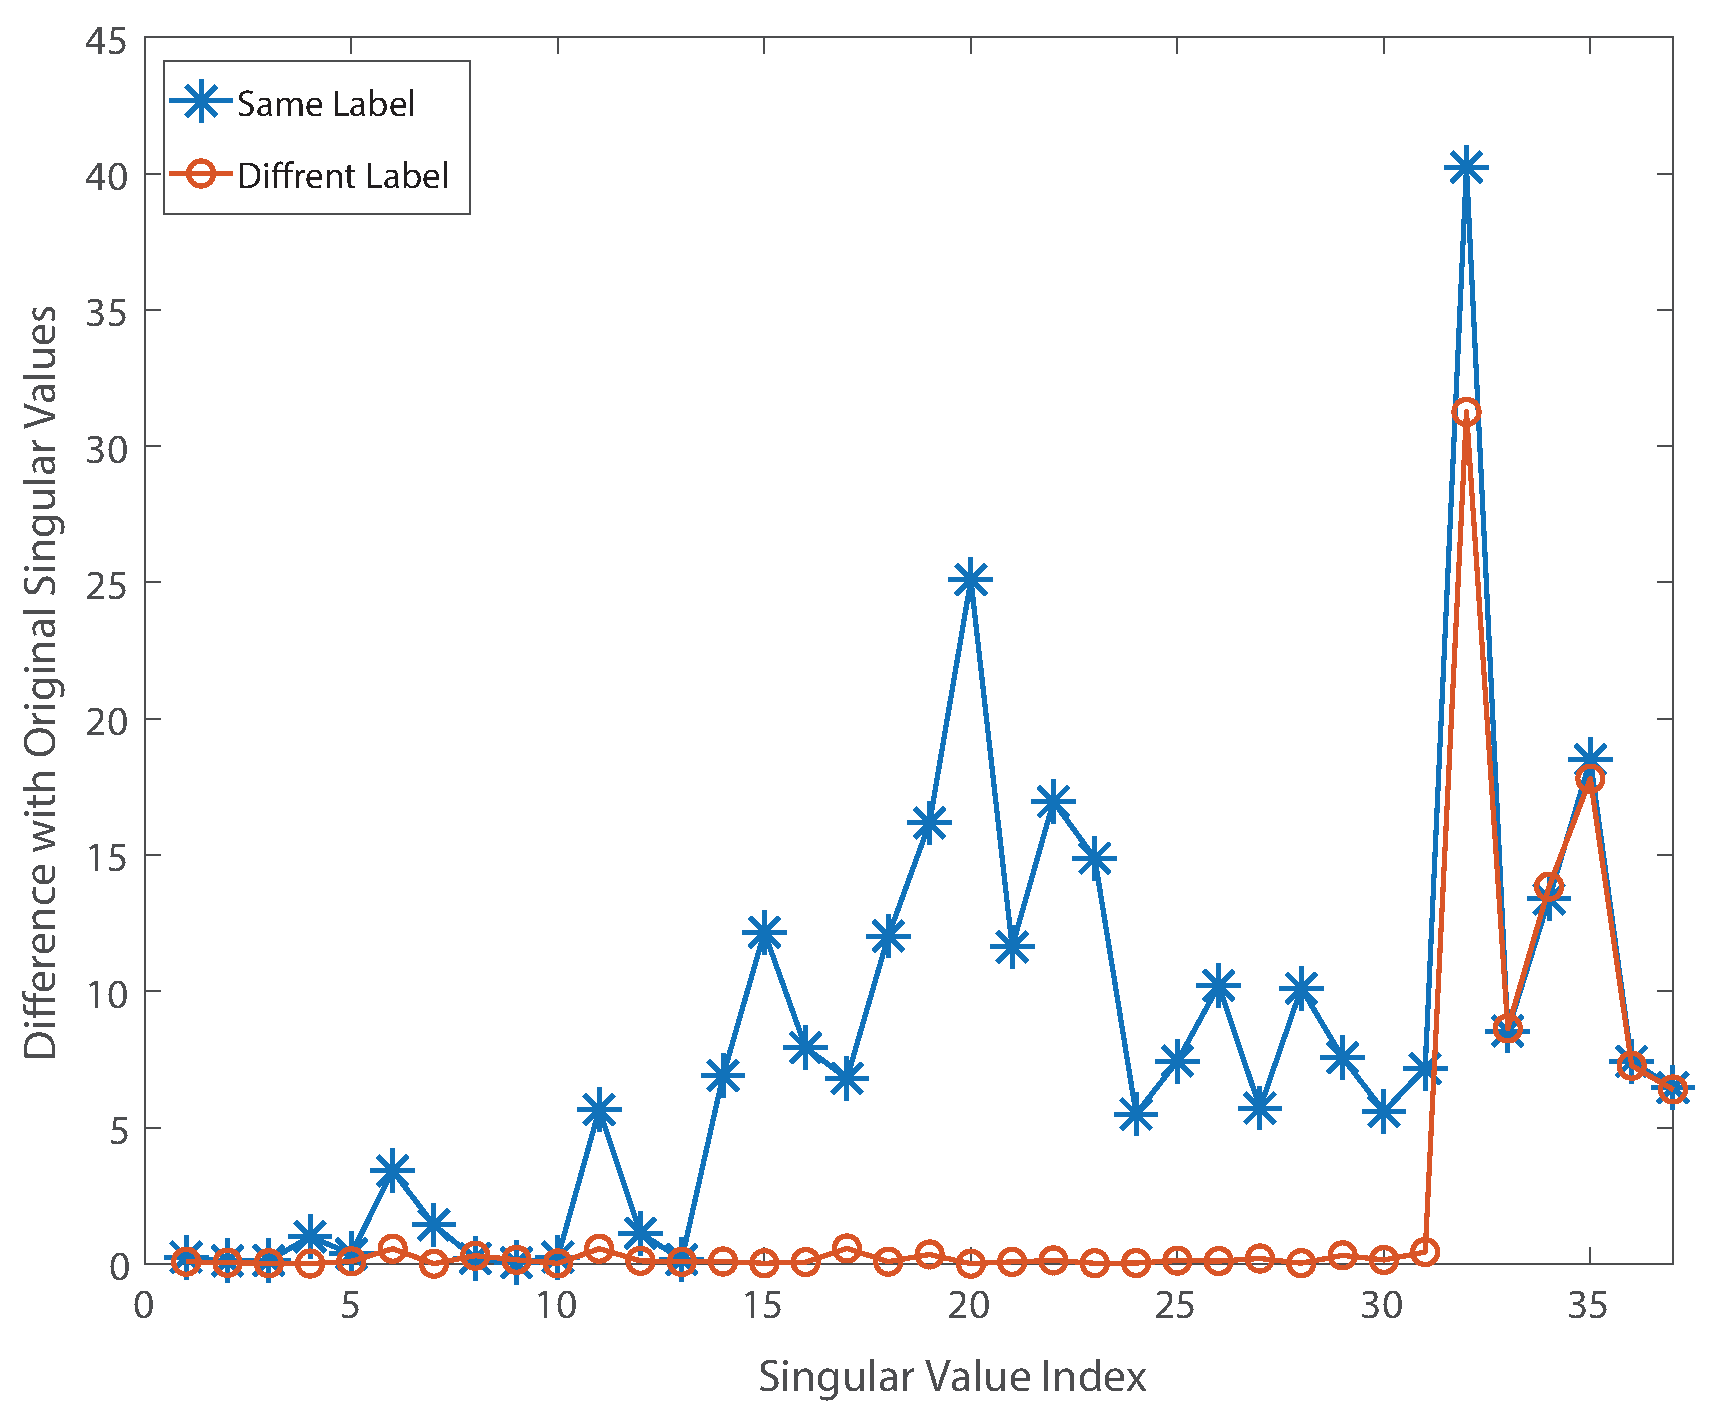
\includegraphics[width=3.5in]{images/SVDiff}
	%		\caption{The blue line with the star indicator, shows the difference between the mode-$3$ singular values of the original data and the data appended with a \emph{same} label subject. The orange line indicated with circles, shows the difference between the mode-$3$ singular values of the original data and the data appended with a \emph{different} label subject.}
	%		\label{g3.1}
	%	\end{figure}
	
	
	%As it was discussed before in \eqref{related_works}, there are two types of FC: Dynamic FC and Static FC. Although the obtained FC is an sFC by definition, we argue that the core tensor obtained from HOSVD, which contains the features included in the FC calculation process, has a dynamic structure. The majority of non-stationary methods uses the sliding window technique in order to analyze the BOLD signal in several sessions. The main idea is that the presence of temporal fluctuations in FC within different sessions should be taken into account in order to obtain a better FC.
	
	\section{EXPERIMENTAL STUDY}
	\subsection{Data Preprocessing and Experimental Settings}
	
	Rs-fMRI data of $196$ subjects were downloaded from the ADNI website\footnote{http://adni.loni.usc.edu}. Nine subjects were discarded
	due to the corruption of data, and the remaining $187$ subjects were preprocessed for analysis. After removing subjects that had problems in the preprocessing steps, such as large head motion,
	$156$ subjects were kept, including $26$ AD, $44$ early MCI, $38$ late MCI, $38$ NC, and ten significant memory concern labeled by ADNI. We used the $38$ NC and the $44$ early MCI because our focus in this paper is to identify MCI at a very early stage, which is the most challenging and significant task in AD
	prediction. The IDs of the $82$ ($38$ NC and $44$ early MCI) subjects are provided in the supplementary material. 
	
	The data are acquired on a $3$-T (Philips) scanner with TR/TE set as $3000/30$
	ms and flip angle of $80◦$. Each series has $140$ volumes, and each volume consists of 48 slices of image matrices with dimensions
	$64 \times 64$
	with voxel size of
	$ 3.31 \times  3.31 \times 3.31$
	$mm^3$ . The preprocessing is carried out using SPM12 and DPARSFA \cite{r64.5}. The
	first ten volumes of each series are discarded for signal equilibrium. Slice timing, head motion correction, and MNI space normalization are performed. Participants with too much head motion are excluded. The normalized brain images are warped into automatic anatomical labeling (AAL) \cite{r64.7} atlas to obtain $116$ ROIs as nodes. By following common practice \cite{n1, n2, n3}, the ROI mean time series are extracted by averaging the time series from all voxels within each ROI and then bandpass filtered to obtain multiple sub-bands as in \cite{n3}. 
	
	\subsection{Classification}
	
	Almost every subject in ADNI dataset has several scans. Usually, random scan data is selected and enters the processing step\cite{r14}. This random selection may cause several problems. Since the number of train data is very low, a small alteration in the samples could drastically change the set of input parameters in order to achieve the highest prediction accuracy and other classification evaluation methods. Also achieving high-quality results with a classifier does not guarantee its effectiveness on other datasets even with fine-tuning the parameters since the training set may contain outliers and unidentified corrupted data.
	
	In order to show that the proposed framework is less sensitive against the choice of different permutations of data (i.e. Same patient with the different scan) is less vulnerable towards the aforementioned issues, we have selected $18$ different permutations of data and test two state of the art classification methods on them: \textbf{HON} and \textbf{k-SICE}.   
	To make full use of the limited subjects, a leave-one-out procedure is used for training and test. That is, each sample is reserved for the test in turn, while the remaining samples are used for training.
	We have use five
	evaluation measures: accuracy (ACC), sensitivity (SEN), Youden’s index(YI), F-score, and balanced accuracy (BAC)\cite{r65}.
	
	%The detailed definitions
	%of these seven statistical measures are provided in Table \eqref{Table_1}, where TP, TN, FP, and FN denote the true positive, true negative, false positive, and false negative, respectively, and 
	%$precision =  \frac{TP}{TP + FP}  $ 
	%and 
	%$recall = \frac{TP}{TP + FN}$.
	In this article, we treat the eMCI samples as positive class and the NC samples as negative class.
	%\begin{table}
	%	\begin{center}
	%			\caption{Definitions of five statistical measurement
	%			indices} \label{Table_1}
	%		\begin{tabular}{l c}
	%			\hline
	%			\hline
	%			Measureement & Definition\\
	%			\hline
	%			\\
	%			Acc & $\dfrac{TP+TN}{TP+FP+TN+FN}$\\[7pt]
	%			SEN & $\dfrac{TP}{TP+FN}$\\[7pt]
	%			%SPE & $\dfrac{TN}{TN+FP}$\\[7pt]
	%			YI & $SEN + SPE - 1$\\[7pt]
	%			F-Score & $2\times \dfrac{precesion \times recall}{precesion + recall}$\\[7pt]
	%			BAC & $\dfrac{1}{2}(SEN + SPE)$\\[7pt]
	%			\hline
	%			\hline
	%		\end{tabular}
	%	\end{center}
	%\end{table}
	
	\subsubsection{Classification performance}
	The classification accuracy measure(ACC), After fine-tuning the input parameter set for each method, shows that for $16$ out of $18$ different random selected datasets, our approach performs better than k-SICE, the same also holds for $15$ datasets comparing to HON. i.e. in $88.8 \%$ of datasets, proposed method works better than k-SICE and in $83.3 \%$ of datasets, it works better than FON.  
	The highest classification accuracy($86.59\%$) is achieved with the proposed method in the $15$th sample data. The highest accuracy for the HON ($84.15\%$) is achieved in the $14$th, and the highest accuracy for the SICE method ($85.37\%$) is achieved in the $6$th sample data. As it was mentioned before, being stable when the input dataset changes is a very important aspect for a classifier, in order to measure the stability, the standard deviation of accuracy along with other measures are
	calculated. The std. of accuracy for the proposed method is $0.64$ times less than HON and $1.73$ times less than k-SICE method. Similar results also hold for other classification measures.
	\begin{figure*}
		\centering
		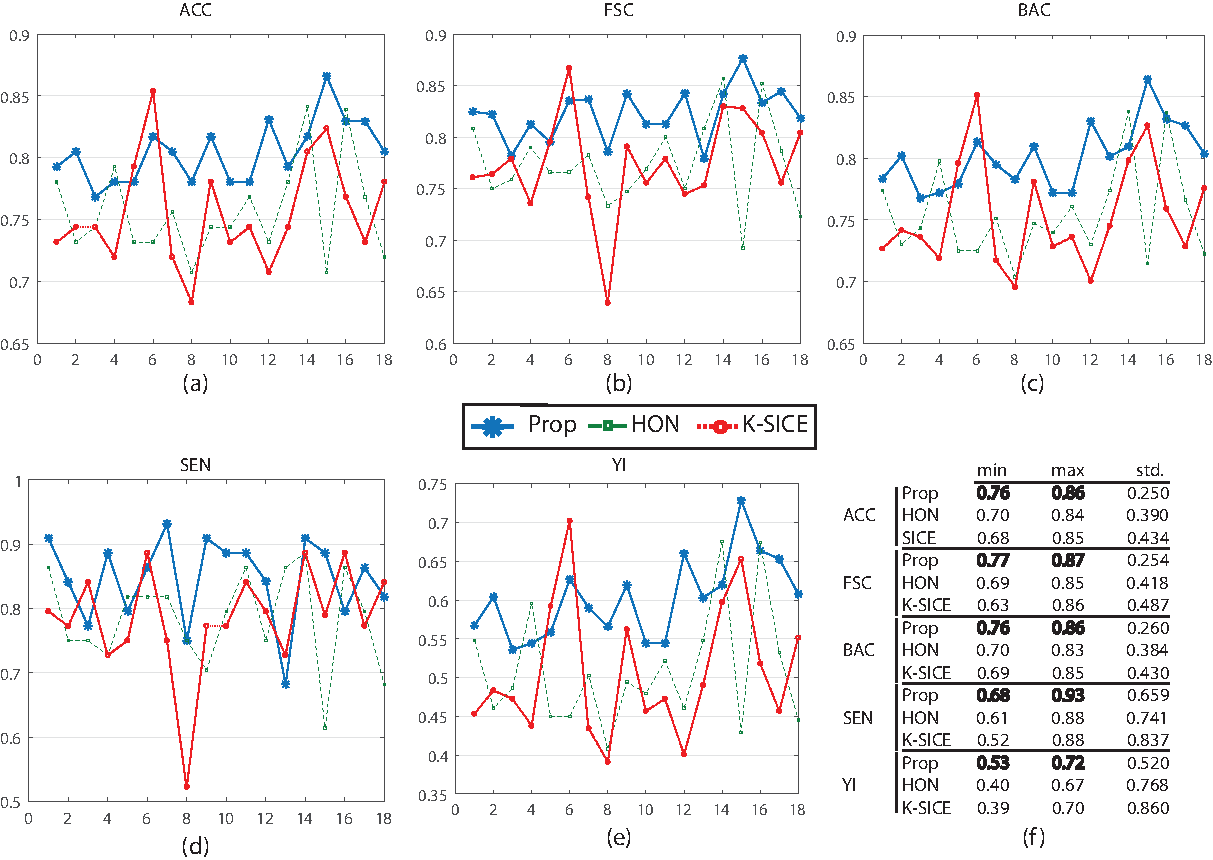
\includegraphics[width=6in]{images/Final-eps.pdf}
		\caption{
			% Updated upstream
			Comparison of proposed method(Prop) with K-SICE and HON 
			applied on 18 different dataset permutations 
			in five different classification evaluation measures.
			Figures \textit{a} through \textit{e} shows \textit{accuracy}, \textit{F-Score}, \textit{balanced accuracy}, \textit{sensitivity} and \textit{Youden Index} respectively
			along with the max, min and standard deviation of each one presented at the embedded table (f). 
			%=======
			%		Comparison of proposed method(Prop) with K-SICE and HON in five different classification evaluation measures along with the standard deviation of each one. %As it can be seen, the both the minimum and maximum of the proposed methods in these measurements are higher that the other two. Also the lower std. of our method indicates its stability.   
			%>>>>>>> Stashed changes
		}
		\label{g3.2}
	\end{figure*}
	
	
	Figure \eqref{g3.2} shows the performance of these three methods in all five measurements. Some statistical information about these plots is also included in the embedded table. As it can bee seen in this figure, similar to the accuracy, the proposed method in overall works much better than FON and k-SICE. For a better Demonstration, table \eqref{AVG} provides the average of several classification measurements scores for all dataset permutations. 
	\begin{table}
		\begin{center}
			\caption{The Average of Different Classification Measurements in all dataset permutations in \% }
			%\resizebox{\textwidth}{!}{  
			\begin{tabular}{@{}c*{6}{c}}
				\hline\hline
				Method&ACC& F-Score&SEN & SPE &YI & BAC 
				\\
				\hline
				k-SICE  &75.57& 77.36 & 78.50 & 72.19 & 50.69 & 75.34 
				\\
				FON   &75.66& 77.44 & 78.40 & 72.48 & 50.89 & 75.44  
				\\
				Proposed &\textbf{80.43}& \textbf{82.20} & \textbf{84.60} & \textbf{75.59} & \textbf{60.20} & \textbf{80.09}
				
				\\
				
				\hline\hline
				\label{AVG}
			\end{tabular}
			%}
		\end{center}
	\end{table}
	As it can be seen in this table, the average accuracy of Proposed method which is $80.43 \%$ is $4.77\%$ higher than the next method HON, and $4.86 \%$ better than k-SICE. It is noteworthy that The other two methods i.e HON and SICE shows similar results in average.  
	
	\begin{figure*}
		\centering
		
\includegraphics[width=6in]{images/FG}
		\caption{
			The difference graph. This graph is obtained via subtracting the functional connectivity of eMCI subjects from normal subjects. Each circle represents a ROI in AAL atlas and the color and size of each circle is proportional to the graph clustering coefficient of the difference graph. red = more activity in EMCI, green: less. 
		}
		\label{g3.3}
	\end{figure*}
	
	\subsubsection{Runtime Comparison}
	One other key features of the proposed method is that it works significantly faster than the other two methods. Table \eqref{Time} shows the average elapsed time (Training plus Testing) of each method for all data permutations. These methods were executed in Matlab R2017b and carried with an Intel Core-i7 processor and $16$GB of RAM. As it can be seen in this table, the proposed method is more than $600$ times faster than HON and $20$ times faster that SICE.   
	\begin{table}
		\begin{center}
			\caption{Elapsed time of the test and train phase in seconds}
			%\resizebox{\textwidth}{!}{  
			\begin{tabular}{@{}c*{4}{c}}
				\hline\hline
				Method& HON & k-SICE& proposed method 
				\\
				\hline
				Elapsed Time  &6950& 230 & 11 
				\\
				\hline\hline
				\label{Time}
			\end{tabular}
			%}
		\end{center}
	\end{table}
	Having a huge execution time especially affects the parameter selection for HON, since it uses cross-validation procedure in order to find the optimal parameters which itself require several runs of the algorithm. 
	%\subsubsection{Parameter Estimation and Sensitivity}
	%As it was discussed before, the choice of parameters drastically affect the performance of the aforementioned classifier. 
	
	
	
	\subsection{Functional connectivity Network}
	The vector features for both Normal and eMCI classes was obtained via the proposed method as it is described in \eqref{FC_Construction}. Due to the aforementioned qualities of partial correlation, SICE is deployed in order to obtain the final FC.  
	In order to better highlight the differences between Normal and eMCI subjects, a difference graph $D$ is constructed by subtracting the Normal FC from the eMCI FC. This graph could be seen in Figure\eqref{g3.3}. 
	The nodes of $D$ shows the ROIs according to the AAL atlas. The size of each node is proportional to its graph clustering coefficient, i.e. the bigger node demonstrates higher activity in eMCI subjects in the corresponding ROI. 
	Similar to nodes, the size of each edge is also proportional to the correlation between two ROI's. In addition, the edges are also color-coded in a way that the green edges show the positive edges in $D$ and the orange edges shows the negative edges in $D$. In this manner, the green edges demonstrate decreasing in activity between the corresponding nodes in eMCI subjects and vice versa, the orange edges shows increasing activity between corresponding ROIs in the eMCI subjects.   
	
	As it can be seen in the difference graph, the big nodes i.e. ROIs with higher activities does not necessarily establish strong connections with the other nodes. As an obvious example, higher activities in Lingual gyrus(ROI index: 47,48)\cite{r25}, Calcarine sulcus(ROI index: 43, 44)\cite{r26,r27}, Supplementary motor area(ROI index: 19,20)\cite{r27,r28} and Temporal\_mid\_L(ROI index: 85)\cite{r29} are easily detectable. The majority of ROIs located in frontal lobe also shows rather high activities comparing to normal subjects\cite{r30,r04}.
	
	Similar to the nodes, the strong edge between two ROIs does not necessarily require the nodes to be highly active in eMCI. Although a strong edge does indicate high activities and functional connectivity between the two corresponding ROIs. The difference Graph shows a significant increase in connectivity between 
	Rectus(ROI index: 28, 27 in Frontal lobe) and 
	Parietal\_Sup\_R(ROI index: 60 in Parietal lobe) \cite{r40, r41},
	Frontal\_Inf\_Orb\_R(ROI index: 16 in Frontal lobe) and
	Cingulum\_Ant(ROI index: 31,32 in Limbic lobe)\cite{r42},
	Insula\_L, Temporal\_Pole\_Sup\_L(ROI index: 29,83 in Limbic lobe) and
	Pallidum\_R, Caudate\_R(ROI index: 29,83 in Sub Cortical Grey Nuclei)\cite{r43}. It can also be seen that within activities in frontal lobe also increased in patients with eMCI\cite{r44}. There is a decrease in connectivity between Amygdala\_L(ROI index: 41 in Sub Cortical Grey Nuclei) with Frontal\_Mid\_Orb\_R(ROI index: 10 in Sub Frontal lobe) and ParaHippocampal\_L(ROI index: 39 in Sub Limbic lobe)\cite{r45}. The connectivity between Heschl\_L(ROI index: 79 in Temporal lobe) and two ROIs Temporal\_Mid\_R(ROI index: 86 also in Temporal lobe) and Occipital\_Inf\_R(ROI index: 54 in Occipital lobe) also decreased in eMCI\cite{r46}. 
	
	\subsubsection*{\textbf{Regarding the Cerebellum and Vermis}}
	In fMRI data analysis and especially in Alzheimer's disease studies, ROIs within the Cerebellum and Vermis are usually excluded since their role was regarded as insignificant\cite{r47, r48}. Recent studies have shown that the traditional assumption that Cerebral area is essential only for the coordination of voluntary motor activity and motor learning is not valid and indicates the significant role of the cerebellum in nervous system function, cognition, and emotion\cite{r32}. 
	
	As it can be seen in the difference graph that we obtained, ROIs within Cerebellum and Vermis are highly active and both their Intra and interconnections are noticeable. There is increased functional connectivity between the Limbic lobe especially 
	Hippocampus\_R, Temporal\_Pole\_Mid(ROI index: 38,87,88)
	and Cerebral areas in eMCI patients. Also, the connectivity between Occipital lobe, especially Occipital\_mid\_R(ROI index: 52), the Frontal lobe, especially in Frontal\_mid\_orb(ROI index: 9,10) and Cerebral areas seems to decrease in patients with eMCI. 
	
	
	
	
	%\begin{table*}
	%	\begin{center}
	%		\caption{Active Nodes }
	%		\resizebox{\textwidth}{!}{  
	%		\begin{tabular}{@{}l*{4}{l}}
	%			\hline\hline
	%			NO.&ROI Index&ROI name&Location& Citations 
	%			\\
	%			\hline
	%			1& 8 & Frontal\_Mid\_R & Middle frontal gyrus
	%			$\rightarrow$ Prefrontal cortex $\rightarrow$ \textbf{Frontal lobe}
	%			 & Main 
	%			\\
	%			2& 14 & Frontal\_Inf\_Tri\_R & Inferior frontal gyrus, pars triangularis
	%			$\rightarrow$ Inferior frontal gyrus $\rightarrow$ Prefrontal cortex
	%			 $\rightarrow$ \textbf{Frontal lobe} & Main 
	%			\\
	%			3& 17 & Rolandic\_Oper\_L & Rolandic operculum
	%			$\rightarrow$ Operculum $\rightarrow$ \textbf{Cerebral cortex} & Main 
	%			\\
	%			4& 19 & Supp\_Motor\_Area\_L & Supplementary motor area
	%			$\rightarrow$ Motor area $\rightarrow$ \textbf{Functional area} & Main 
	%			\\
	%			5& 20 & Supp\_Motor\_Area\_R & Supplementary motor area
	%			$\rightarrow$ Motor area $\rightarrow$ \textbf{Functional area} & Main 
	%			\\
	%			6& 25 & Frontal\_Med\_Orb\_L &  Medial orbitofrontal cortex $\rightarrow$ Orbitofrontal cortex
	%			$\rightarrow$ Orbitofrontal area $\rightarrow$ \textbf{Frontal lobe} & ? 
	%			\\
	%			7 & 34 & Cingulum\_Mid\_R & Right midcingulate area
	%			$\rightarrow$ Midcingulate area $\rightarrow$ Cingulate gyrus
	%			$\rightarrow$ Cerebral cortex $\rightarrow$ \textbf{Frontal lobe} & ? 
	%			\\
	%			8 & 43 & Calcarine\_L & Calcarine sulcus
	%			$\rightarrow$ Midcingulate area $\rightarrow$ \textbf{Sulcus} & ? 
	%			\\
	%			9 & 44 & Calcarine\_R & Calcarine sulcus
	%			$\rightarrow$ Midcingulate area $\rightarrow$ \textbf{Sulcus} & ? 
	%			\\
	%			10 & 47 & Lingual\_L & Lingual gyrus
	%			$\rightarrow$ Occipital lobe $\rightarrow$Cerebral cortex $\rightarrow$ \textbf{Frontal lobe} & ? 
	%			\\
	%			11 & 48 & Lingual\_R & Lingual gyrus
	%			$\rightarrow$ Occipital lobe $\rightarrow$Cerebral cortex $\rightarrow$ \textbf{Frontal lobe} & ? 
	%			\\
	%			12 & 70 & Paracentral\_Lobule\_R & Paracentral lobule $\rightarrow$ \textbf{Frontal lobe} & ?
	%			\\
	%			13 & 69 & Paracentral\_Lobule\_L & Middle temporal gyrus $\rightarrow$ \textbf{Temporal lobe} & ?
	%			\\
	%			14 & 99 & Cerebelum\_6\_L & Lobule VI of cerebellar hemisphere $\rightarrow$Cerebellum
	%			$\rightarrow$ Metencephalon $\rightarrow$ \textbf{Hindbrain} & ?
	%			\\
	%			15 & 111 & Vermis\_4\_5 & Vermis $\rightarrow$ Cerebellum $\rightarrow$ Metencephalon $\rightarrow$ \textbf{Hindbrain} & ?
	%			\\
	%			\hline\hline
	%			\label{sss}
	%		\end{tabular}
	%		}
	%	\end{center}
	%\end{table*}
	
	
	
	
	% An example of a floating figure using the graphicx package.
	% Note that \label must occur AFTER (or within) \caption.
	% For figures, \caption should occur after the \includegraphics.
	% Note that IEEEtran v1.7 and later has special internal code that
	% is designed to preserve the operation of \label within \caption
	% even when the captionsoff option is in effect. However, because
	% of issues like this, it may be the safest practice to put all your
	% \label just after \caption rather than within \caption{}.
	%
	% Reminder: the "draftcls" or "draftclsnofoot", not "draft", class
	% option should be used if it is desired that the figures are to be
	% displayed while in draft mode.
	%
	%\begin{figure}[!t]
	%\centering
	%\includegraphics[width=2.5in]{myfigure}
	% where an .eps filename suffix will be assumed under latex, 
	% and a .pdf suffix will be assumed for pdflatex; or what has been declared
	% via \DeclareGraphicsExtensions.
	%\caption{Simulation results for the network.}
	%\label{fig_sim}
	%\end{figure}
	
	% Note that the IEEE typically puts floats only at the top, even when this
	% results in a large percentage of a column being occupied by floats.
	
	
	% An example of a double column floating figure using two subfigures.
	% (The subfig.sty package must be loaded for this to work.)
	% The subfigure \label commands are set within each subfloat command,
	% and the \label for the overall figure must come after \caption.
	% \hfil is used as a separator to get equal spacing.
	% Watch out that the combined width of all the subfigures on a 
	% line do not exceed the text width or a line break will occur.
	%
	%\begin{figure*}[!t]
	%\centering
	%\subfloat[Case I]{\includegraphics[width=2.5in]{box}%
	%\label{fig_first_case}}
	%\hfil
	%\subfloat[Case II]{\includegraphics[width=2.5in]{box}%
	%\label{fig_second_case}}
	%\caption{Simulation results for the network.}
	%\label{fig_sim}
	%\end{figure*}
	%
	% Note that often IEEE papers with subfigures do not employ subfigure
	% captions (using the optional argument to \subfloat[]), but instead will
	% reference/describe all of them (a), (b), etc., within the main caption.
	% Be aware that for subfig.sty to generate the (a), (b), etc., subfigure
	% labels, the optional argument to \subfloat must be present. If a
	% subcaption is not desired, just leave its contents blank,
	% e.g., \subfloat[].
	
	
	% An example of a floating table. Note that, for IEEE style tables, the
	% \caption command should come BEFORE the table and, given that table
	% captions serve much like titles, are usually capitalized except for words
	% such as a, an, and, as, at, but, by, for, in, nor, of, on, or, the, to
	% and up, which are usually not capitalized unless they are the first or
	% last word of the caption. Table text will default to \footnotesize as
	% the IEEE normally uses this smaller font for tables.
	% The \label must come after \caption as always.
	%
	%\begin{table}[!t]
	%% increase table row spacing, adjust to taste
	%\renewcommand{\arraystretch}{1.3}
	% if using array.sty, it might be a good idea to tweak the value of
	% \extrarowheight as needed to properly center the text within the cells
	
	
	
	
	
	
	
	
	
	
	
	
	
	
	
	
	
	
	
	
	
	
	
	
	%\caption{An Example of a Table}
	%\label{table_example}
	%\centering
	%% Some packages, such as MDW tools, offer better commands for making tables
	%% than the plain LaTeX2e tabular which is used here.
	%\begin{tabular}{|c||c|}
	%\hline
	%One & Two\\
	%\hline
	%Three & Four\\
	%\hline
	%\end{tabular}
	%\end{table}
	
	
	% Note that the IEEE does not put floats in the very first column
	% - or typically anywhere on the first page for that matter. Also,
	% in-text middle ("here") positioning is typically not used, but it
	% is allowed and encouraged for Computer Society conferences (but
	% not Computer Society journals). Most IEEE journals/conferences use
	% top floats exclusively. 
	% Note that, LaTeX2e, unlike IEEE journals/conferences, places
	% footnotes above bottom floats. This can be corrected via the
	% \fnbelowfloat command of the stfloats package.
	
	
	
	
	\section{Conclusion}
	The majority of functional connectivity analysis methods rely on calculating the FC matrix for each individual, then using simple methods to combine them in order to obtain a general FC network for a class. Also, the state of the art classification techniques  use FC as the representative for each sample. In this paper, based on multilinear nature of data, we have proposed a novel framework in which the general FC is extracted directly from the Time-Region features  and does not rely on individual FC calculations. Also the obtained FC by the proposed method contains some relations that recently  approved 
	experimentally.
	This framework also ables us to design a discriminant function that works directly with $Time \times  Region$ samples rather that their FC. The new discriminant function also uses the test data in order to enhance the training set. The benefits of the proposed method could be summarize as follow: 
	%\begin{enumerate}
	%Taking advantage of multilinear nature of data, Avoid vectorization at any stage, 
	%	\item FC calculation regarding the whole class
	%	\item Directly classifying the original $Time \times  Region$ matrix
	%	\item Uses test samples to enhance the training set
	%\end{enumerate}  
	Extensive studies on the rs-fMRI provided by ADNI shows the superiority of the proposed framework in both classification and functional connectivity. The obtained FC network not only acknowledge the previous discovered connections but also reveals new connectivity patterns previously unknown.
	The framework proposed in this paper can be easily extended to other studies involved with high order data.  
	
	%\begin{table*}
	%	\begin{center}
	%		\caption{content...}
	%		\resizebox{\textwidth}{!}{  
	%	\begin{tabular}{@{}c*{20}{c}}
	%		\hline\hline
	%		\multicolumn{20}{c}{Datasets} 
	%		\\
	%		\hline
	%&\multicolumn{1}{|c}{TBNA} & \textbf{79.27} & \textbf{80.49} & \textbf{76.83} & 78.05 & 78.05 & 81.71 & \textbf{80.49} & \textbf{78.05} & \textbf{81.71} & \textbf{78.05} & \textbf{78.05} & \textbf{83.1} & \textbf{79.27} & 8171 & \textbf{86.59} & 82.93 & \textbf{82.93} & \textbf{80.49} 
	%\\
	%ACC&\multicolumn{1}{|c}{FON} & 78.05 & 73.17 & 74.39 & \textbf{79.27} & 73.17 & 73.17 & 75.61 & 70.73 & 74.39 & 74.39 & 76.83 & 73.17 & 78.05 & \textbf{84.15} & 70.73 & \textbf{83.9} & 76.83 & 71.95 
	%\\
	%&\multicolumn{1}{|c}{SICE} & 73.17 & 74.39 & 74.39 & 71.95 & \textbf{79.27} & \textbf{85.37} & 71.95 & 68.29 & 78.05 & 73.17 & 74.39 & 70.73 & 74.39 & 80.49 & 82.38 & 76.83 & 73.17 & 78.05 
	%%\\\hline
	%%&\multicolumn{1}{|c}{TBNA} & \textbf{0.9091} & \textbf{0.8409} & 0.7727 & \textbf{0.8864} & 0.7955 & \textbf{0.8636} & \textbf{0.9318} & 0.75 & \textbf{0.9091} & \textbf{0.8864} & \textbf{0.8864} & \textbf{0.8421} & 0.6818 & \textbf{0.9091} & \textbf{0.8864} &\textbf{ 0.7955} &\textbf{ 0.8636} & \textbf{0.8182} 
	%%\\
	%%SEN&\multicolumn{1}{|c}{FON} & 0.8636 & 0.75 & 0.75 & 0.7273 & \textbf{0.8182} & 0.8182 & 0.8182 & 0.75 & 0.7045 & 0.7955 & 0.8636 & 0.75 & \textbf{0.8636} & 0.8864 & 0.6136 & 0.8636 & 0.7955 & 0.6818 
	%%\\
	%%&\multicolumn{1}{|c}{SICE} & 0.7955 & 0.7727 & \textbf{0.8409} & 0.7273 & 0.75 & 0.8864 & 0.75 & 0.5227 & 0.7727 & 0.7727 & 0.8409 & 0.7955 & 0.7273 & 0.8864 & 0.7895 & 0.8864 & 0.7727 & 0.8409 
	%\\\hline
	%%&\multicolumn{1}{|c}{TBNA} & 0.6579 & \textbf{0.7632} & \textbf{0.7632} & 0.6579 & \textbf{0.7632} & 0.7632 & 0.6579 & 0.8158 & 0.7105 & 0.6579 & 0.6579 & 0.8182 & 0.9211 & 0.7105 & 0.8421 & 0.8684 & 0.7895 & 0.7895 
	%%\\
	%%SPE&\multicolumn{1}{|c}{FON} & 0.6842 & 0.7105 & 0.7368 & 0.8684 & 0.6316 & 0.6316 & 0.6842 & 0.6579 & 0.7895 & 0.6842 & 0.6579 & 0.7105 & 0.6842 & 0.7895 & 0.8158 & 0.8106 & 0.7368 & 0.7632 
	%%\\
	%%&\multicolumn{1}{|c}{SICE} & 0.6579 & 0.7105 & 0.6316 & 0.7105 & 0.8421 & 0.8158 & 0.6842 & 0.8684 & 0.7895 & 0.6842 & 0.6316 & 0.6053 & 0.7632 & 0.7105 & 0.8636 & 0.6316 & 0.6842 & 0.7105 
	%%\\\hline
	%%&\multicolumn{1}{|c}{TBNA} & 0.567 & 0.6041 & 0.5359 & 0.5443 & 0.5586 & 0.6268 & 0.5897 & 0.5658 & 0.6196 & 0.5443 & 0.5443 & 0.6603 & 0.6029 & 0.6196 & 0.7285 & 0.6639 & 0.6531 & 0.6077 
	%%\\
	%%YI&\multicolumn{1}{|c}{FON} & 0.5478 & 0.4605 & 0.4868 & 0.5957 & 0.4498 & 0.4498 & 0.5024 & 0.4079 & 0.494 & 0.4797 & 0.5215 & 0.4605 & 0.5478 & 0.6758 & 0.4294 & 0.6742 & 0.5323 & 0.445 
	%%\\
	%%&\multicolumn{1}{|c}{SICE} & 0.4533 & 0.4833 & 0.4725 & 0.4378 & 0.5921 & 0.7022 & 0.4342 & 0.3911 & 0.5622 & 0.4569 & 0.4725 & 0.4007 & 0.4904 & 0.5969 & 0.6531 & 0.5179 & 0.4569 & 0.5514 
	%%\\\hline
	%&\multicolumn{1}{|c}{TBNA} &\textbf{ 82.47} & \textbf{82.22} & \textbf{78.16} & \textbf{81.25} & \textbf{79.55} & 83.52 & \textbf{83.67} &\textbf{ 78.57} & \textbf{84.21} & \textbf{81.25 } & \textbf{81.25} & \textbf{84.25} & 77.92 & 84.21 & \textbf{87.64 }& 83.33 & \textbf{84.44} & \textbf{81.82 }
	%\\
	%F-SC&\multicolumn{1}{|c}{FON} & 80.85 & 75 & 75.86 & 79.01 & 76.6 & 76.6 & 78.26 & 73.33 & 74.7 & 76.92 & 80 & 75 & \textbf{80.85} & \textbf{85.71} & 69.23 & \textbf{85.2} & 78.65 & 72.29 
	%\\
	%&\multicolumn{1}{|c}{SICE} & 76.09 & 76.4 & 77.89 & 73.56 & 79.52 & \textbf{86.67} & 74.16 & 63.89 & 79.07 & 75.56 & 77.89 & 74.47 & 75.29 & 82.98 & 82.79 & 80.41 & 75.56 & 80.43 
	%\\\hline
	%%&\multicolumn{1}{|c}{TBNA} & 0.7835 & 0.802 & 0.7679 & 0.7721 & 0.7793 & 0.8134 & 0.7949 & 0.7829 & 0.8098 & 0.7721 & 0.7721 & 0.8301 & 0.8014 & 0.8098 & 0.8642 & 0.8319 & 0.8266 & 0.8038 
	%%\\
	%%BAC&\multicolumn{1}{|c}{FON} & 0.7739 & 0.7303 & 0.7434 & 0.7978 & 0.7249 & 0.7249 & 0.7512 & 0.7039 & 0.747 & 0.7398 & 0.7608 & 0.7303 & 0.7739 & 0.8379 & 0.7147 & 0.8371 & 0.7661 & 0.7225 
	%%\\
	%%&\multicolumn{1}{|c}{SICE} & 0.7267 & 0.7416 & 0.7362 & 0.7189 & 0.7961 & 0.8511 & 0.7171 & 0.6956 & 0.7811 & 0.7285 & 0.7362 & 0.7004 & 0.7452 & 0.7984 & 0.8266 & 0.759 & 0.7285 & 0.7757 
	%%		& HON & &\multicolumn{1}{|c}{kernel} & \\
	%%		
	%%		& TBNA & &\multicolumn{1}{|c}{kernel} & \\
	%		 \\
	%		\hline\hline
	%	\end{tabular}
	%}
	%	\end{center}
	%\end{table*}
	
	
	
	
	
	
	
	% if have a single appendix:
	%\appendix[Proof of the Zonklar Equations]
	% or
	%\appendix  % for no appendix heading
	% do not use \section anymore after \appendix, only \section*
	% is possibly needed
	
	% use appendices with more than one appendix
	% then use \section to start each appendix
	% you must declare a \section before using any
	% \subsection or using \label (\appendices by itself
	% starts a section numbered zero.)
	%
	
	
	%\appendices
	%\section{Proof of the First Zonklar Equation}
	%Appendix one text goes here.
	
	% you can choose not to have a title for an appendix
	% if you want by leaving the argument blank
	%\section{}
	%Appendix two text goes here.
	
	
	%	% use section* for acknowledgment
	%	\section*{Acknowledgment}
	%	
	%	
	%	The authors would like to thank...
	
	
	% Can use something like this to put references on a page
	% by themselves when using endfloat and the captionsoff option.
	%\ifCLASSOPTIONcaptionsoff
	%\newpage
	%\fi
	
	
	
	% trigger a \newpage just before the given reference
	% number - used to balance the columns on the last page
	% adjust value as needed - may need to be readjusted if
	% the document is modified later
	%\IEEEtriggeratref{8}
	% The "triggered" command can be changed if desired:
	%\IEEEtriggercmd{\enlargethispage{-5in}}
	
	% references section
	
	% can use a bibliography generated by BibTeX as a .bbl file
	% BibTeX documentation can be easily obtained at:
	% http://mirror.ctan.org/biblio/bibtex/contrib/doc/
	% The IEEEtran BibTeX style support page is at:
	% http://www.michaelshell.org/tex/ieeetran/bibtex/
	%\bibliographystyle{IEEEtran}
	% argument is your BibTeX string definitions and bibliography database(s)
	%\bibliography{IEEEabrv,../bib/paper}
	%
	% <OR> manually copy in the resultant .bbl file
	% set second argument of \begin to the number of references
	% (used to reserve space for the reference number labels box)			
	
	
	%% The Appendices part is started with the command \appendix;
	%% appendix sections are then done as normal sections
	%% \appendix
	
	%% \section{}
	%% \label{}
	
	%% References
	%%
	%% Following citation commands can be used in the body text:
	%% Usage of \cite is as follows:
	%%   \cite{key}         ==>>  [#]
	%%   \cite[chap. 2]{key} ==>> [#, chap. 2]
	%%
	
	%% References with bibTeX database:
	
	
	
	
	
	
	
	%\bibliographystyle{elsarticle-num}
	%\bibliography{<your-bib-database>}
	
	%% Authors are advised to submit their bibtex database files. They are
	%% requested to list a bibtex style file in the manuscript if they do
	%% not want to use elsarticle-num.bst.
	
	%% References without bibTeX database:
	
	% \begin{thebibliography}{00}
	
	%% \bibitem must have the following form:
	%%   \bibitem{key}...
	%%
	
	% \bibitem{}
	
	% \end{thebibliography}
	
	%\section{Bibliography}
	\begin{thebibliography}{1}
		
		\bibitem{r01}
		Caselli, Richard J., et al. "Longitudinal changes in cognition and behavior in asymptomatic carriers of the APOE e4 allele." Neurology 62.11 (2004): 1990-1995.
		
		\bibitem{r02}
		Brookmeyer, Ron, et al. "Forecasting the global burden of Alzheimer’s disease." Alzheimer's \& dementia: the journal of the Alzheimer's Association 3.3 (2007): 186-191.
		
		\bibitem{r03}
		Musha, Toshimitsu, et al. "EEG markers for characterizing anomalous activities of cerebral neurons in NAT (neuronal activity topography) method." IEEE Transactions on Biomedical Engineering 60.8 (2013): 2332-2338.
		
		\bibitem{r21}
		Nordberg, Agneta. "PET imaging of amyloid in Alzheimer's disease." The lancet neurology 3.9 (2004): 519-527.
		
		\bibitem{r22}
		Jeong, Jaeseung. "EEG dynamics in patients with Alzheimer's disease." Clinical neurophysiology 115.7 (2004): 1490-1505.
		
		\bibitem{r23}Golby, Alexandra, et al. "Memory encoding in Alzheimer's disease: an fMRI study of explicit and implicit memory." Brain 128.4 (2005): 773-787.
		
		
		
%		\bibitem{r04}
%		Gould, R. L., et al. "Brain mechanisms of successful compensation during learning in Alzheimer disease." Neurology 67.6 (2006): 1011-1017.
		
		\bibitem{r04}Dennis, Emily L., and Paul M. Thompson. "Functional brain connectivity using fMRI in aging and Alzheimer’s disease." Neuropsychology review 24.1 (2014): 49-62.
		
		%		\bibitem{r05}
		%		Richiardi, Jonas, et al. "Classifying minimally disabled multiple sclerosis patients from resting state functional connectivity." Neuroimage 62.3 (2012): 2021-2033.
		
		%		\bibitem{r06}
		%		Yang, Xue, et al. "Evaluation of statistical inference on empirical resting state fMRI." IEEE Transactions on Biomedical Engineering 61.4 (2014): 1091-1099.
		
		\bibitem{r07}
		R. Graaf and K. Kevin. Methods and apparatus for
		compensating eld inhomogeneities in magnetic resonance
		studies. US Patent No. 8035387, 2011.
		
			\bibitem{r33}N. Leonardi et al., “Principal components of functional connectivity: A
		new approach to study dynamic brain connectivity during rest,” NeuroImage,
		vol. 83, pp. 937–950, 2013.
		
		\bibitem{r34}Cherkassky, Vladimir L., et al. "Functional connectivity in a baseline resting-state network in autism." Neuroreport 17.16 (2006): 1687-1690.
		
		%		\bibitem{r08}
		%		Zhang, Xiaowei, et al. "Resting-state whole-brain functional connectivity networks for mci classification using l2-regularized logistic regression." IEEE transactions on nanobioscience 14.2 (2015): 237-247.
		
		\bibitem{r09}
		Stanley, Matthew Lawrence, et al. "Defining nodes in complex brain networks." Frontiers in computational neuroscience 7 (2013): 169.
		
		
		\bibitem{r35}Du, Yuhui, Zening Fu, and Vince D. Calhoun. "Classification and prediction of brain disorders using functional connectivity: promising but challenging." Frontiers in neuroscience 12 (2018).
		
		\bibitem{r36}de Vos, Frank, et al. "A comprehensive analysis of resting state fMRI measures to classify individual patients with Alzheimer's disease." Neuroimage 167 (2018): 62-72.
		
		
			\bibitem{r37}Cuingnet, Rémi, et al. "Automatic classification of patients with Alzheimer's disease from structural MRI: a comparison of ten methods using the ADNI database." neuroimage 56.2 (2011): 766-781.
		
		
		\bibitem{r38}Friston, Karl J. "Functional and effective connectivity: a review." Brain connectivity 1.1 (2011): 13-36.
		
		
		\bibitem{r55}Leonardi, Nora, et al. "Principal components of functional connectivity: a new approach to study dynamic brain connectivity during rest." NeuroImage 83 (2013): 937-950.
		
		\bibitem{r53}Supekar, Kaustubh, et al. "Network analysis of intrinsic functional brain connectivity in Alzheimer's disease." PLoS computational biology 4.6 (2008): e1000100.
		
		\bibitem{r54}Contreras, Joey A., et al. "Resting state network modularity along the prodromal late onset Alzheimer's disease continuum." NeuroImage: Clinical 22 (2019): 101687.
		
		\bibitem{r60}Ahmadi, Soheil, and Mansoor Rezghi. "A novel extension of Generalized Low-Rank Approximation of Matrices based on multiple-pairs of transformations." CoRR (2018).
		
		
		\bibitem{r10}
		Jie, Biao, et al. "Integration of network topological and connectivity properties for neuroimaging classification." IEEE transactions on biomedical engineering 61.2 (2014): 576-589.
		
		
	
		
		
	
		
		\bibitem{r11}
		Wee, Chong-Yaw, et al. "Resting-state multi-spectrum functional connectivity networks for identification of MCI patients." PloS one 7.5 (2012): e37828.
		
		\bibitem{r12}
		Tibshirani, Robert, et al. "Sparsity and smoothness via the fused lasso." Journal of the Royal Statistical Society: Series B (Statistical Methodology) 67.1 (2005): 91-108.
		
		
		
		\bibitem{r13}
		Wright, John, et al. "Robust face recognition via sparse representation." IEEE transactions on pattern analysis and machine intelligence 31.2 (2009): 210-227.
		
		\bibitem{r15}
		Huang, Shuai, et al. "Learning brain connectivity of Alzheimer's disease by sparse inverse covariance estimation." NeuroImage 50.3 (2010): 935-949.
		
		
		\bibitem{r16}
		Allen, Elena A., et al. "Tracking whole-brain connectivity dynamics in the resting state." Cerebral cortex 24.3 (2014): 663-676.
		
		\bibitem{r19}
		Leonardi, Nora, et al. "Principal components of functional connectivity: a new approach to study dynamic brain connectivity during rest." NeuroImage 83 (2013): 937-950.
		
		\bibitem{r56}Leonardi, Nora, and Dimitri Van De Ville. "On spurious and real fluctuations of dynamic functional connectivity during rest." Neuroimage 104 (2015): 430-436.
		
		
		\bibitem{r58}Barttfeld, Pablo, et al. "Signature of consciousness in the dynamics of resting-state brain activity." Proceedings of the National Academy of Sciences 112.3 (2015): 887-892.
		
		\bibitem{r59}Zalesky, Andrew, et al. "Time-resolved resting-state brain networks." Proceedings of the National Academy of Sciences 111.28 (2014): 10341-10346.
		
			\bibitem{r57}
		Hindriks, Rikkert, et al. "Can sliding-window correlations reveal dynamic functional connectivity in resting-state fMRI?." Neuroimage 127 (2016): 242-256.
		
		\bibitem{r61}Ng, Bernard, et al. "A novel sparse group Gaussian graphical model for functional connectivity estimation." International Conference on Information Processing in Medical Imaging. Springer, Berlin, Heidelberg, 2013.
		
		
		
		\bibitem{r62}Colclough, Giles L., et al. "Multi-subject hierarchical inverse covariance modelling improves estimation of functional brain networks." NeuroImage 178 (2018): 370-384.
		
		\bibitem{r63}	Foti, Nicholas J., and Emily B. Fox. "Statistical model-based approaches for functional connectivity analysis of neuroimaging data." Current opinion in neurobiology 55 (2019): 48-54.	
		
		
		
		\bibitem{r14}
		Zhang, Jianjia, et al. "Functional brain network classification with compact representation of SICE matrices." IEEE Transactions on Biomedical Engineering 62.6 (2015): 1623-1634.
		
		
		
		
		\bibitem{r49}V.Arsigny et al.,. (2006). Log-euclidean metrics for fast and simple calculus
		on diffusion tensors. Magn. Reson. Med.. [Online]. 56(2), pp. 411–421.
		Available: http://dx.doi.org/10.1002/mrm.20965
		
		\bibitem{r50}S. Sra, “A new metric on the manifold of kernel matrices with application
		to matrix geometric mean,” in Advances in Neural Information Processing
		Systems 25, F. Pereira, C. J. C. Burges, L. Bottou, K. Q.Weinberger, Eds.,
		New York, NY: Curran Associates, Inc., 2012, pp. 144–152.
		
		\bibitem{r63.5}Chen, Xiaobo, et al. "High‐order resting‐state functional connectivity network for MCI classification." Human brain mapping 37.9 (2016): 3282-3296.
		
		\bibitem{r64}Rezghi, Mansoor. "A novel fast tensor-based preconditioner for image restoration." IEEE Transactions on Image Processing 26.9 (2017): 4499-4508.
		
		
		\bibitem{r64.5}Yan, Chaogan, and Yufeng Zang. "DPARSF: a MATLAB toolbox for" pipeline" data analysis of resting-state fMRI." Frontiers in systems neuroscience 4 (2010): 13.
		
		
		\bibitem{r64.7}Tzourio-Mazoyer, Nathalie, et al. "Automated anatomical labeling of activations in SPM using a macroscopic anatomical parcellation of the MNI MRI single-subject brain." Neuroimage 15.1 (2002): 273-289.
		
		
		\bibitem{n1}S. M. Smith et al., “Functional connectomics from resting-state fMRI,”
		Trends Cognit. Sci., vol. 17, no. 12, pp. 666–682, 2013.
		
		\bibitem{n2}N. Leonardi et al., “Principal components of functional connectivity: A
		new approach to study dynamic brain connectivity during rest,” NeuroImage,
		vol. 83, pp. 937–950, 2013.
		
		\bibitem{n3}C.-Y. Wee et al., “Constrained sparse functional connectivity networks
		for MCI classification,” in Proc. Med. Image Comput. Comput.-Assisted
		Intervention Conf., 2012, pp. 212–219.
		
		\bibitem{r65}Tan, Pang-Ning. Introduction to data mining. Pearson Education India, 2018.
		
		%%%*/*/*/*/*/*/*/*/*/ HERE HRRE
		
		%		\bibitem{r17}
		%		Damaraju, Eswar, et al. "Dynamic functional connectivity analysis reveals transient states of dysconnectivity in schizophrenia." NeuroImage: Clinical 5 (2014): 298-308.
		
		%		\bibitem{r18}
		%		Hutchison, R. Matthew, et al. "Dynamic functional connectivity: promise, issues, and interpretations." Neuroimage 80 (2013): 360-378.
		
		
		
		%		\bibitem{r20}
		%		Leonardi, Nora, et al. "Principal components of functional connectivity: a new approach to study dynamic brain connectivity during rest." NeuroImage 83 (2013): 937-950.
		
		
		
		\bibitem{r25}He, Yong, et al. "Regional coherence changes in the early stages of Alzheimer’s disease: a combined structural and resting-state functional MRI study." Neuroimage 35.2 (2007): 488-500.
		
		
		
		\bibitem{r26}Bakkour, Akram, et al. "The effects of aging and Alzheimer's disease on cerebral cortical anatomy: specificity and differential relationships with cognition." Neuroimage 76 (2013): 332-344.
		
		\bibitem{r27}Brewer, Alyssa A., and Brian Barton. "Visual cortex in aging and Alzheimer's disease: changes in visual field maps and population receptive fields." Frontiers in psychology 5 (2014): 74.
		
		\bibitem{r28}Jacobsen, Jörn-Henrik, et al. "Why musical memory can be preserved in advanced Alzheimer’s disease." Brain 138.8 (2015): 2438-2450.
		
		\bibitem{r29}Kosicek, Marko, and Silva Hecimovic. "Phospholipids and Alzheimer’s disease: alterations, mechanisms and potential biomarkers." International journal of molecular sciences 14.1 (2013): 1310-1322.
		
		\bibitem{r30}Salvatore, Christian, et al. "Magnetic resonance imaging biomarkers for the early diagnosis of Alzheimer's disease: a machine learning approach." Frontiers in neuroscience 9 (2015): 307.
		
		
		\bibitem{r32}Jacobs, Heidi IL, et al. "The cerebellum in Alzheimer’s disease: evaluating its role in cognitive decline." Brain 141.1 (2017): 37-47.
		
	
		
		
		
		
		
		
		
		
		
		%		\bibitem{r39}Jones, David T., et al. "Non-stationarity in the “resting brain’s” modular architecture." PloS one 7.6 (2012): e39731.
		
		\bibitem{r40}Brickman, Adam M., et al. "Reconsidering harbingers of dementia: progression of parietal lobe white matter hyperintensities predicts Alzheimer's disease incidence." Neurobiology of aging 36.1 (2015): 27-32.
		
		\bibitem{r41}De Reuck, J., et al. "Topography of cortical microbleeds in Alzheimer’s disease with and without cerebral amyloid angiopathy: a post-mortem 7.0-tesla MRI Study." Aging and disease 6.6 (2015): 437.
		
		\bibitem{r42}Perani, Daniela, et al. "The impact of bilingualism on brain reserve and metabolic connectivity in Alzheimer's dementia." Proceedings of the National Academy of Sciences 114.7 (2017): 1690-1695.
		
		\bibitem{r43}Watson, Rosie, et al. "Subcortical volume changes in dementia with Lewy bodies and Alzheimer's disease. A comparison with healthy aging." International psychogeriatrics 28.4 (2016): 529-536.
		
		\bibitem{r44}Cai, Suping, et al. "Changes in thalamic connectivity in the early and late stages of amnestic mild cognitive impairment: a resting-state functional magnetic resonance study from ADNI." PloS one 10.2 (2015): e0115573.
		
		\bibitem{r45}Ortner, Marion, et al. "Progressively Disrupted intrinsic Functional connectivity of Basolateral amygdala in Very early alzheimer’s Disease." Frontiers in neurology 7 (2016): 132.
		
		\bibitem{r46}Steketee, Rebecca ME, et al. "Early-stage differentiation between presenile Alzheimer’s disease and frontotemporal dementia using arterial spin labeling MRI." European radiology 26.1 (2016): 244-253.
		
		\bibitem{r47}Sanz-Arigita, Ernesto J., et al. "Loss of ‘small-world’networks in Alzheimer's disease: graph analysis of FMRI resting-state functional connectivity." PloS one 5.11 (2010): e13788.
		
		\bibitem{r48}Zhang, Daoqiang, et al. "Multimodal classification of Alzheimer's disease and mild cognitive impairment." Neuroimage 55.3 (2011): 856-867.
		
		
		\bibitem{r51}Allen, Elena A., et al. "Tracking whole-brain connectivity dynamics in the resting state." Cerebral cortex 24.3 (2014): 663-676.
		
		\bibitem{r51}Chang, Catie, and Gary H. Glover. "Time–frequency dynamics of resting-state brain connectivity measured with fMRI." Neuroimage 50.1 (2010): 81-98.
		
		\bibitem{r52}Handwerker, Daniel A., et al. "Periodic changes in fMRI connectivity." Neuroimage 63.3 (2012): 1712-1719.
		
		
		
		
		
	
		
		
		
		
		
		
		
		
		
		
		
		
		
	\end{thebibliography}
	
\end{document}

%%
%% End of file `elsarticle-template-num.tex'.
